%\documentclass[handout]{beamer}
\documentclass{beamer}
\usepackage[utf8]{inputenc}
\usepackage[T1]{fontenc}
\usepackage{xcolor}
%
% Command definitions
%
\newcommand{\problemdomain}{\Omega}
\newcommand{\primalgrid}{\mathcal{G}}
\newcommand{\dualgrid}{\mathcal{\tilde{G}}}
\newcommand{\positionvec}{\bm{r}}
\newcommand{\normal}{\field{n}}
\newcommand{\field}[1]{\bm{#1}}
\newcommand{\fieldfunc}[1]{\field{#1}(\positionvec)}
\newcommand{\tensor}[1]{\field{#1}}
\newcommand{\tensorfunc}[1]{\tensor{#1}(\positionvec)}
\newcommand{\rot}{\nabla\times}
\newcommand{\faradayneumann}{\rot\fieldfunc{e} = -i\omega\fieldfunc{b}}
\newcommand{\amperemaxwell}{\rot\fieldfunc{h} = i\omega\fieldfunc{d} + \fieldfunc{j}_s}
\newcommand{\primaledge}{e}
\newcommand{\primalface}{f}
\newcommand{\dualedge}{\tilde{e}}
\newcommand{\dualface}{\tilde{f}}
\newcommand{\borderprimaledge}{e^b}
\newcommand{\borderdualedge}{\tilde{e}^b}
\newcommand{\primalcurl}{\mathbf{C}}
\newcommand{\dualcurl}{\mathbf{C}^T}
\newcommand{\numatrix}{\mathbf{M}_{\nu}}
\newcommand{\epsmatrix}{\mathbf{M}_{\epsilon}}
\newcommand{\ximatrix}{\mathbf{M}_{\xi}}
\newcommand{\mumatrix}{\mathbf{M}_{\mu}}
\newcommand{\ymatrix}{\mathbf{M}_{Y}}
\newcommand{\mmf}{\mathbf{F}}
\newcommand{\emf}{\mathbf{U}}
\newcommand{\magflux}{\mathbf{\Phi}}
\newcommand{\elecflux}{\mathbf{\Psi}}
\newcommand{\bordermmf}{{\mmf^b}}
\newcommand{\borderemf}{{\emf}}
\newcommand{\basepropagation}{(\dualcurl\numatrix\primalcurl - \omega^2\epsmatrix)\emf}
\newcommand{\basepropagationcompl}{(\dualcurl\ximatrix\primalcurl - \omega^2\mumatrix)\mmf}
\newcommand{\admittancecontrib}{i\omega\ymatrix\emf}
\newcommand{\scatteringborder}{{\partial_s}}
\newcommand{\port}{\Sigma}
\newcommand{\YCalculationPlane}{\Pi}


% Note command:
%  parameter 1: author
%  parameter 2: note text
%\newcommand{\note}[2]{
%    \begin{center}
%        \centering
%        \fcolorbox{red}{YellowGreen}{
%            \mbox{
%                \parbox{0.8\linewidth}{
%                    \begin{center}
%                        \leftpointright~~\textbf{NOTE}
%                    \end{center}
%                    {\footnotesize
%                        \textcolor{red}{\emph{Author:}} #1\\
%                    #2
%                    }
%                }
%            }
%        }
%    \end{center}
%}

% Correction command:
%  parameter 1: author
%  parameter 2: subject
%  parameter 3: status
\newcommand{\correction}[3]{
    \begin{center}
        \centering
        \fcolorbox{red}{GreenYellow}{
            \mbox{
                \parbox{0.8\linewidth}{
                    \begin{center}
                        \smallpencil~~\textbf{CORRECTION}
                    \end{center}
                    {\footnotesize
                        \textcolor{red}{\emph{Proposed by:}} #1\\
                        \textcolor{red}{\emph{Subject:}} #2\\
                        \textcolor{red}{\emph{Status:}} #3\\
                    }
                }
            }
        }
    \end{center}
}



\usepackage{pgfgantt}

\usepackage{tikz}
\usetikzlibrary{arrows}
\usetikzlibrary{patterns}

%\title{Formulazione geometrica discreta per la modellazione nel dominio della frequenza di siti EMC}
\title{Modelling of EMC sites using the Frequency Domain Discrete Geometric Approach\\\phantom{xxx}}
\date{Phd conference 2015}
\author{Matteo Cicuttin}

\usetheme{uniud}

\begin{document}

%%%%%%%%%%%%%%%%%%%%%%%%%%%%%%%%%%%%%%%%%%%%%%%%%%%%
\begin{frame}
\titlepage
\end{frame}

%%%%%%%%%%%%%%%%%%%%%%%%%%%%%%%%%%%%%%%%%%%%%%%%%%%%
\begin{frame}{Activities in the past 30 months}
    Aim: Study and development of numerical models useful to validate and predict the outcome of EMC measurements.
    \begin{figure}
        \centering
        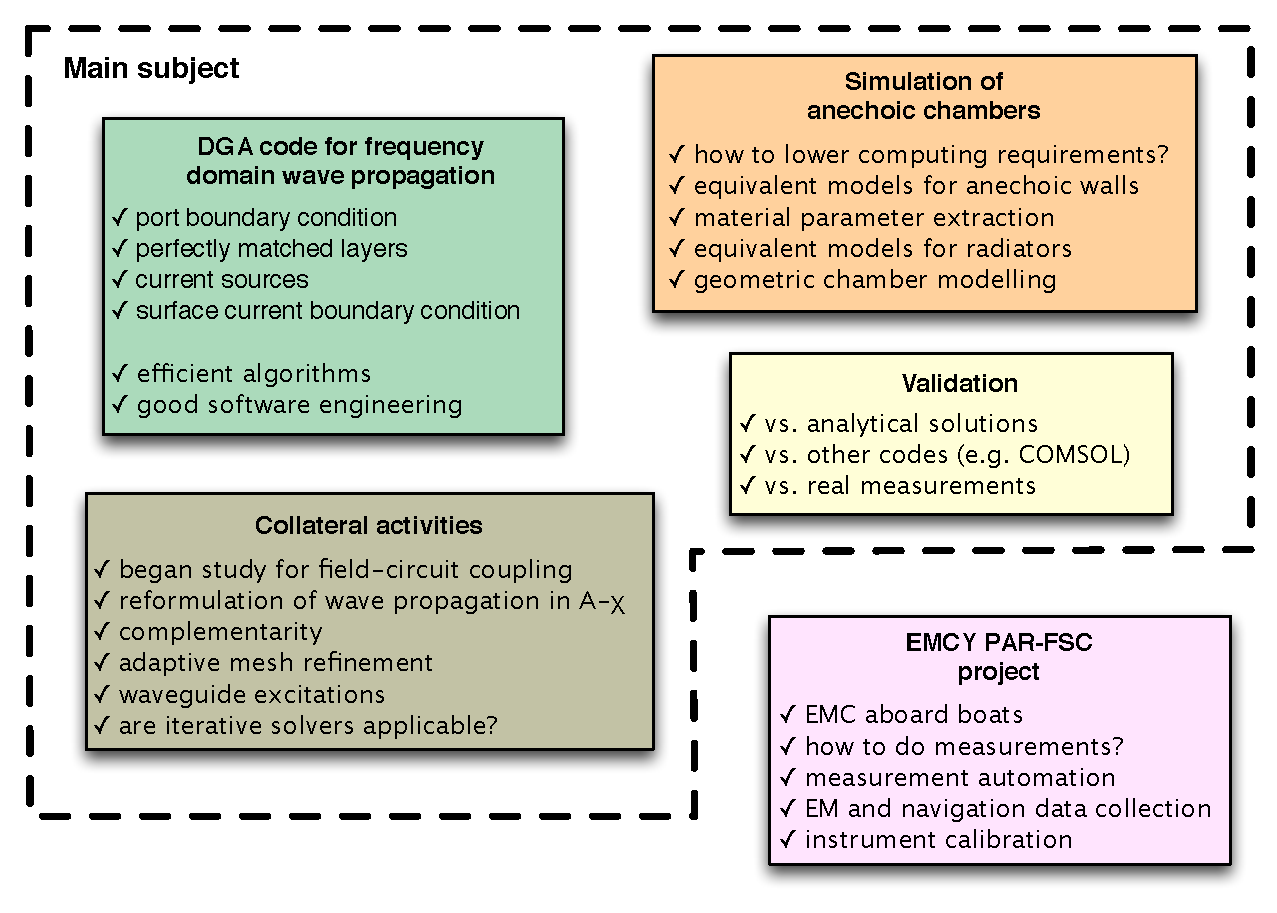
\includegraphics[width=0.85\textwidth]{img/activities.pdf}
    \end{figure}
\end{frame}

%%%%%%%%%%%%%%%%%%%%%%%%%%%%%%%%%%%%%%%%%%%%%%%%%%%%
\begin{frame}{Why these models are useful?}
    Electromagnetic compatibility is a central topic in the development of an electronic product.
    \vspace{5mm}

    \begin{minipage}{0.45\textwidth}
        The test lab:
        \begin{itemize}
            \item Must be sure about the efficiency of the measurement chain
            \item Must be confident about the correctness of the procedures
        \end{itemize}
    \end{minipage}
    \begin{minipage}{0.45\textwidth}
        The manifacturer:
        \begin{itemize}
            \item Must comply with regulations
            \item No recipes to meet required standards
            \item Lab time to debug the products is very costly
        \end{itemize}
    \end{minipage}

    \vspace{5mm}
    Simulation can help with these issues, we'll see how. 
    
    \textcolor{uniud-orange}{Actual demand by the industry.}

\end{frame}


%%%%%%%%%%%%%%%%%%%%%%%%%%%%%%%%%%%%%%%%%%%%%%%%%%%%
\begin{frame}{What is the DGA?}
    The \textcolor{blue}{D}iscrete \textcolor{blue}{G}eometric \textcolor{blue}{A}pproach is a method to solve partial differential equations arising from physics.

    \pause
    \vspace{5mm}
    \begin{minipage}{0.45\textwidth}
    {\scriptsize The domain is discretized in two grids: primal grid \textcolor{blue}{$\mathcal{G}$} and dual grid \textcolor{red}{$\mathcal{\tilde{G}}$}}

    \begin{center}
        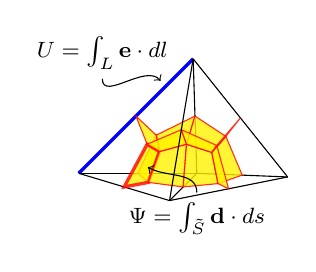
\begin{tikzpicture}[scale=0.3]
            \path [very thick,blue] (0,0,0) edge (6,6,3); %%%%
            \path (0,0,0) edge (5,0,3);
            \path (0,0,0) edge (5,0,0);
            \path (6,6,3) edge (5,0,0);
            \path (5,0,3) edge (5,0,0);
            \path (6,6,3) edge (10,1,3);
            \path (5,0,3) edge (10,1,3);
            \path (5,0,0) edge (10,1,3);
            \filldraw [draw=red,fill=yellow,opacity=8.000000e-01] (3.66667,2,1)--(2.5,0,0)--(3.33333,0,1)--(4,1.5,1.5)--cycle;
            \filldraw [draw=red,fill=yellow,opacity=8.000000e-01] (3.66667,2,1)--(5.5,3,1.5)--(5.33333,2,2)--(4,1.5,1.5)--cycle;
            \filldraw [draw=red,fill=yellow,opacity=8.000000e-01] (3.66667,2,1)--(3,3,1.5)--(3.66667,2,2)--(4,1.5,1.5)--cycle;
            %%%%%%%%%%%%%%%%
            \filldraw [very thick,draw=red,fill=yellow,opacity=8.000000e-01] (3.33333,0,1)--(2.5,0,1.5)--(3.66667,2,2)--(4,1.5,1.5)--cycle;
            %%%%%%%%%%%%%%%%
            \filldraw [draw=red,fill=yellow,opacity=8.000000e-01] (5.33333,2,2)--(5,0,1.5)--(3.33333,0,1)--(4,1.5,1.5)--cycle;
            \filldraw [draw=red,fill=yellow,opacity=8.000000e-01] (3.66667,2,2)--(5.5,3,3)--(5.33333,2,2)--(4,1.5,1.5)--cycle;
            \filldraw [draw=red,fill=yellow,opacity=8.000000e-01] (7,2.33333,2)--(7.5,0.5,1.5)--(6.66667,0.333333,2)--(6.5,1.75,2.25)--cycle;
            \filldraw [draw=red,fill=yellow,opacity=8.000000e-01] (7,2.33333,2)--(5.5,3,1.5)--(5.33333,2,2)--(6.5,1.75,2.25)--cycle;
            \filldraw [draw=red,fill=yellow,opacity=8.000000e-01] (5.33333,2,2)--(5,0,1.5)--(6.66667,0.333333,2)--(6.5,1.75,2.25)--cycle;
            \filldraw [draw=red,fill=yellow,opacity=8.000000e-01] (7,2.33333,3)--(7.5,0.5,3)--(6.66667,0.333333,2)--(6.5,1.75,2.25)--cycle;
            \filldraw [draw=red,fill=yellow,opacity=8.000000e-01] (7,2.33333,3)--(5.5,3,3)--(5.33333,2,2)--(6.5,1.75,2.25)--cycle;
            \filldraw [draw=red,fill=yellow,opacity=8.000000e-01] (7,2.33333,3)--(8,3.5,3)--(7,2.33333,2)--(6.5,1.75,2.25)--cycle;
            \path (6,6,3) edge (5,0,3);

            \node[anchor=south] (e) at (1,4) {\footnotesize $U=\int_L\mathbf{e} \cdot dl$};
            \node[anchor=west] (ee) at (3.4,3.5) {};
            \draw (e) edge[out=270,in=130,->] (ee);

            \node[anchor=south] (j) at (5,-3) {\footnotesize $\Psi=\int_{\tilde{S}}\mathbf{d} \cdot ds$};
            \node[anchor=west] (jj) at (2.1,0.5) {};
            \draw (j) edge[out=90,in=330,->] (jj);
        \end{tikzpicture}
    \end{center}
{\scriptsize An integral quantity is associated to points, lines, surfaces and volumes of each grid}
\end{minipage}
\hfill
\begin{minipage}{0.53\textwidth}
        \scriptsize
        \pause
        Differential operators become incidence matrices (exact)
        \begin{itemize}
            \item $\nabla \implies \mathbf{G}$: node-edge incidence
            \item $\nabla\times \implies \mathbf{C}$: edge-face incidence
            \item $\nabla\cdot \implies \mathbf{D}$: face-volume incidence
        \end{itemize}

        \vspace{1mm}

        \pause
        Primal and dual quantities are related by constitutive matrices (approximate)
        \begin{itemize}
            \item $\mathbf{d} = \epsilon\,\mathbf{e} \implies \Psi = M_{\epsilon} U$ 
            \item $\mathbf{h} = \nu\,\mathbf{b} \implies F = M_{\nu} \Phi$ 
        \end{itemize}
        
        \vspace{1mm}

        \pause
        Discrete equations and continuous equations are very similar
        \begin{itemize}
            \item $\mathbf{e} = -\nabla V \implies U = -\mathbf{G}V$
            \item $\nabla\cdot\mathbf{d} = \rho \implies \mathbf{G}^T\Psi = Q$
            \item $-\nabla\cdot\epsilon\nabla V = \rho \implies -\mathbf{G}^T M_{\epsilon}\mathbf{G}V = Q$
        \end{itemize}

\end{minipage}




\end{frame}

%%%%%%%%%%%%%%%%%%%%%%%%%%%%%%%%%%%%%%%%%%%%%%%%%%%%
\begin{frame}{The code}
    A code for the DGA method was developed. But why?
    \begin{itemize}
        \item Commercial codes don't allow customization, impossibile to test our reseach with them
        \item Commercial codes use FEM, which is different from DGA
    \end{itemize}
    The main features of the new code are
    \begin{itemize}
        \item Modern: it is written in C++14
        \item Modular, expandable and understandable
        \item Fast and highly parallel
        \item General: it is a framework for DGA, not only for frequency domain wave propagation
    \end{itemize}
    The code, which name is EMT, is the foundation for all the subsequent work.
\end{frame}

%%%%%%%%%%%%%%%%%%%%%%%%%%%%%%%%%%%%%%%%%%%%%%%%%%%%
\begin{frame}{The code}
    The wave propagation module of the code has most of the features available in commercial codes.
    \begin{itemize}
        \item Problem specification (\texttt{fdprop} module):
        \begin{itemize}
            \item Port boundary condition (or \emph{plane wave excitation})
            \item Impedance boundary condition (or \emph{radiation condition})
            \item Current sources
            \item Surface current boundary condition
        \end{itemize}
        \item Input/output:
        \begin{itemize}
            \item Graphical output to VisIt and GNUPLOT
        \end{itemize}
    \end{itemize}
    Moreover, it has the features used in the \emph{Equivalent modeling of anechoic chambers}, the subject of my thesis.
\end{frame}

%%%%%%%%%%%%%%%%%%%%%%%%%%%%%%%%%%%%%%%%%%%%%%%%%%%%
\begin{frame}{Simulation of anechoic chambers}
    Simulating an anechoic chamber is a challenging topic.
    \begin{itemize}
        \pause
        \item Problem matrix is indefinite: no iterative solvers!
        \pause
    \item Anechoic chambers are big: \textcolor{green}{lots of elements}
        \pause
    \item Frequencies are high: \textcolor{orange}{more elements}
        \pause
    \item There are antennas inside the chamber, which have fine geometric details: \textcolor{red}{too many elements}
    \end{itemize}

    \pause
    \vspace{3mm}
    With Intel MKL Pardiso and a machine with 32 GB of RAM the limit is about 1.3M equations (In-core).

    \vspace{3mm}
    How to reduce computational requirements?

\end{frame}


%%%%%%%%%%%%%%%%%%%%%%%%%%%%%%%%%%%%%%%%%%%%%%%%%%%%%%%%%%%%%%%%%%%%%%%%%%%%%%%%
\begin{frame}{Equivalent model for anechoic walls}
    \begin{minipage}{0.55\textwidth}

        \only<1>{The anechoic wall model is obtained by studying the basic unit of an anechoic wall, the \emph{unitary cell}.
            \begin{itemize}
                \item 2 $\times$ 2 cones
                \item 3 $\times$ 3 ferrite tiles
            \end{itemize}
            Our goal is to try to remove the cones and the ferrites and substitute them with an impedance boundary condition.    
        }

        \only<2->{A port boundary condition had to be developed to study the unitary cell. The idea is:
        \begin{itemize}
            \onslide<2->{\item use the port to apply a plane wave on $\port$}
            \onslide<3->{\item calculate wave impedance on a plane far away from cones}
            \onslide<4->{\item translate impedance on the rightmost end of the cell}
            \onslide<5->{\item substitute cones and ferrites with that equivalent impedance}
        \end{itemize}
        }
        %\begin{figure}
        %    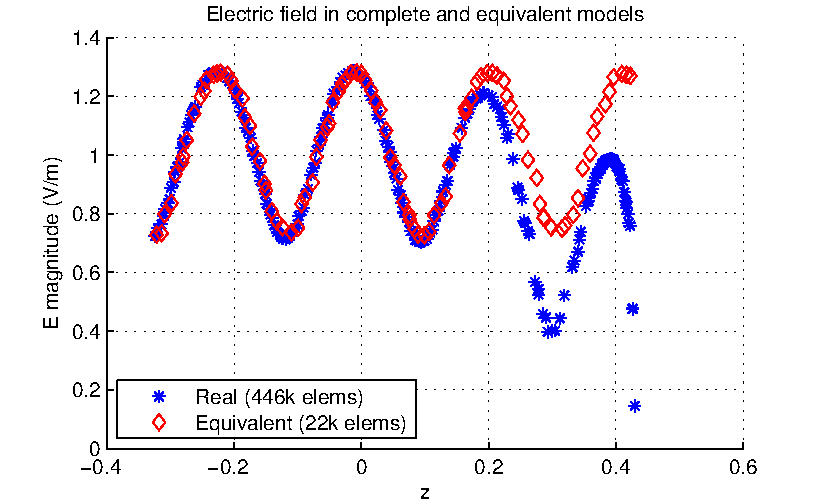
\includegraphics[width=0.45\textwidth]{img/efield_cmp_2.pdf}
        %    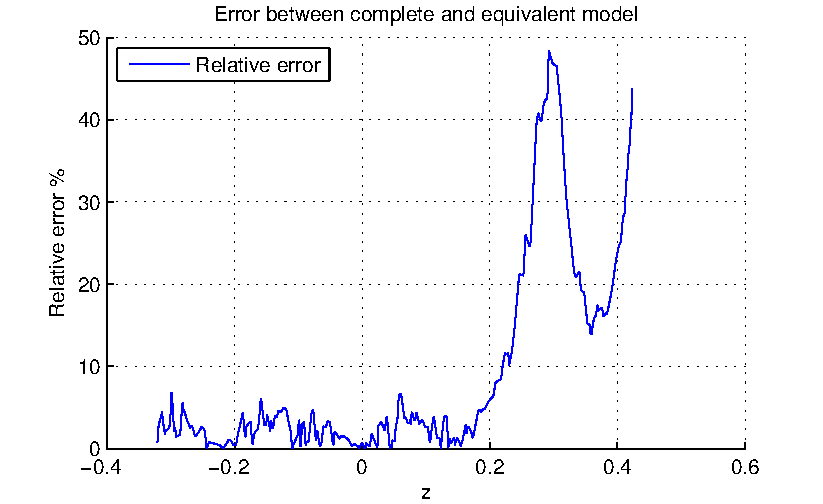
\includegraphics[width=0.45\textwidth]{img/error_2.pdf}
        %\end{figure}

    \end{minipage}
    \begin{minipage}{0.43\textwidth}
        \setbeamercovered{invisible}
        \only<1>{
        \begin{figure}
            \centering
            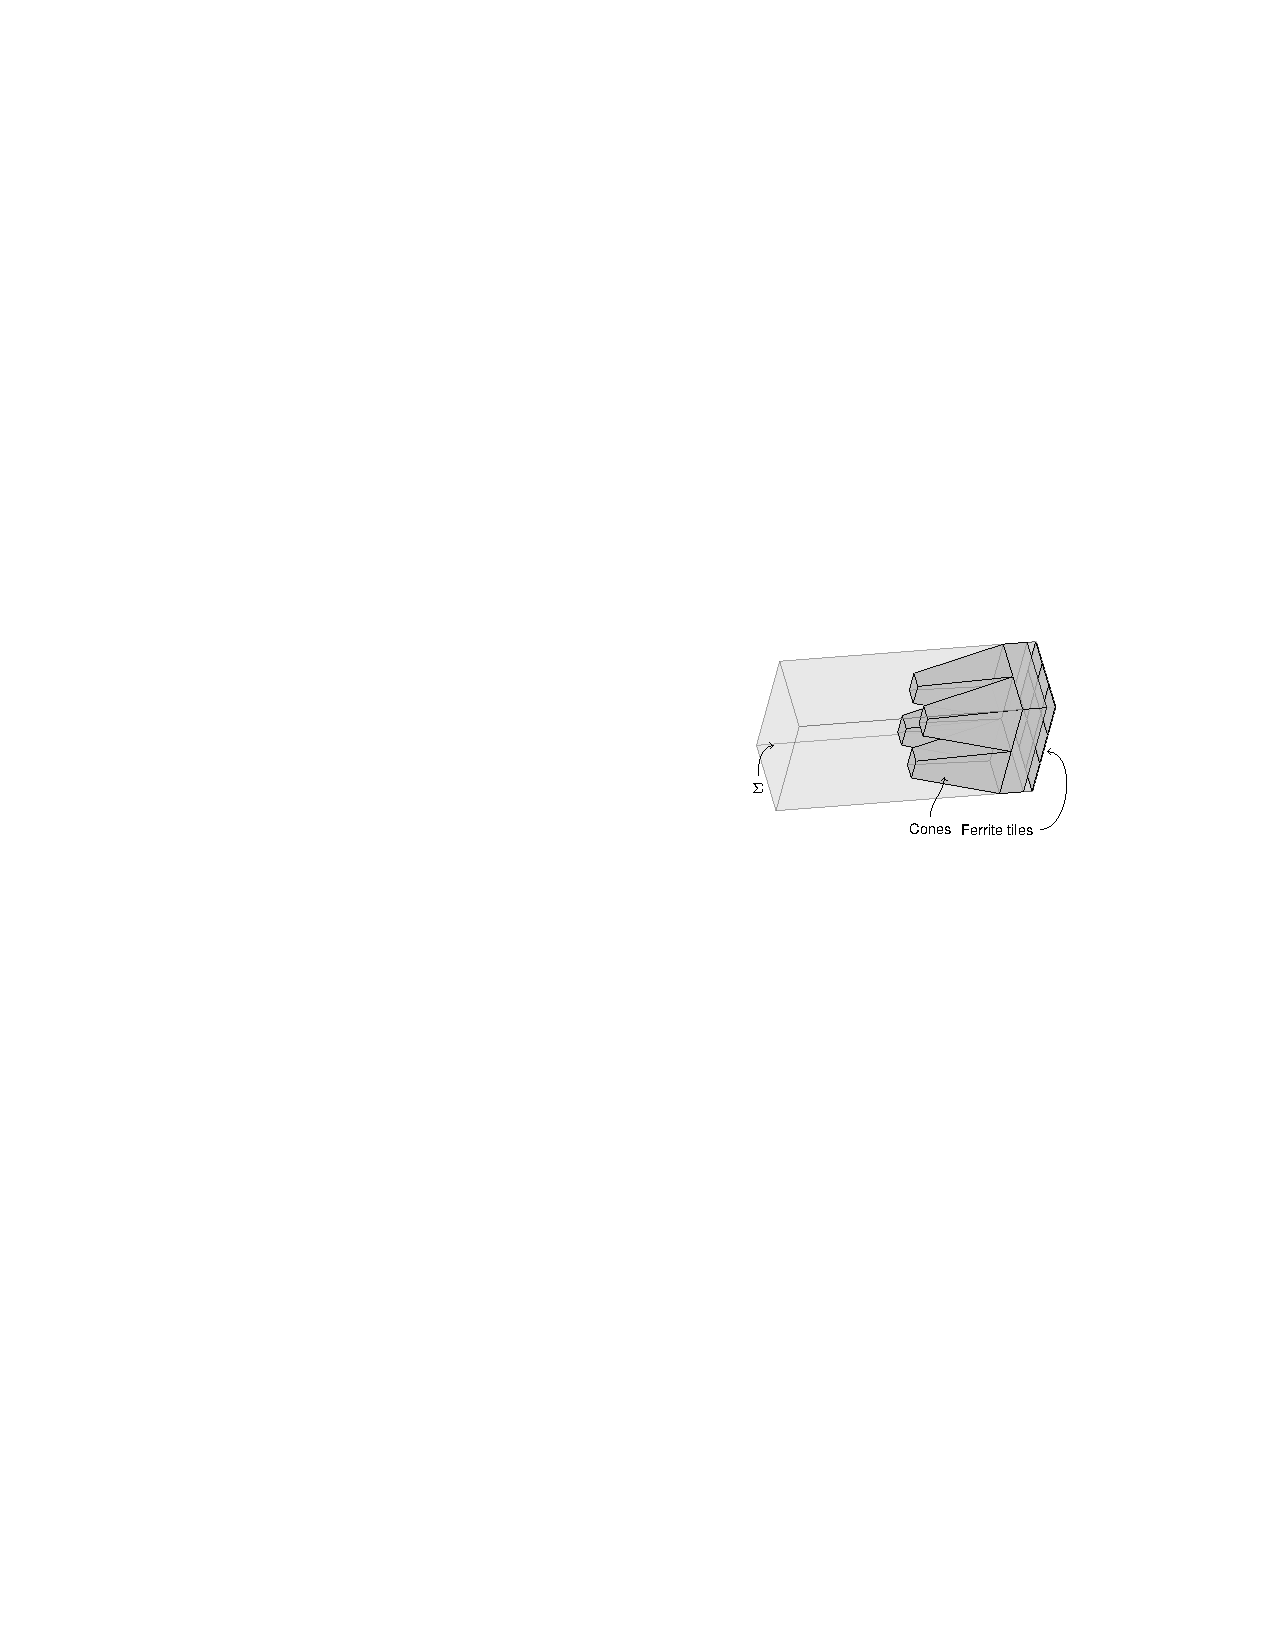
\includegraphics[width=0.9\textwidth]{img/unitcell.pdf}
        \end{figure}
        }

        \only<2->{
            \begin{figure}
                \onslide<2->{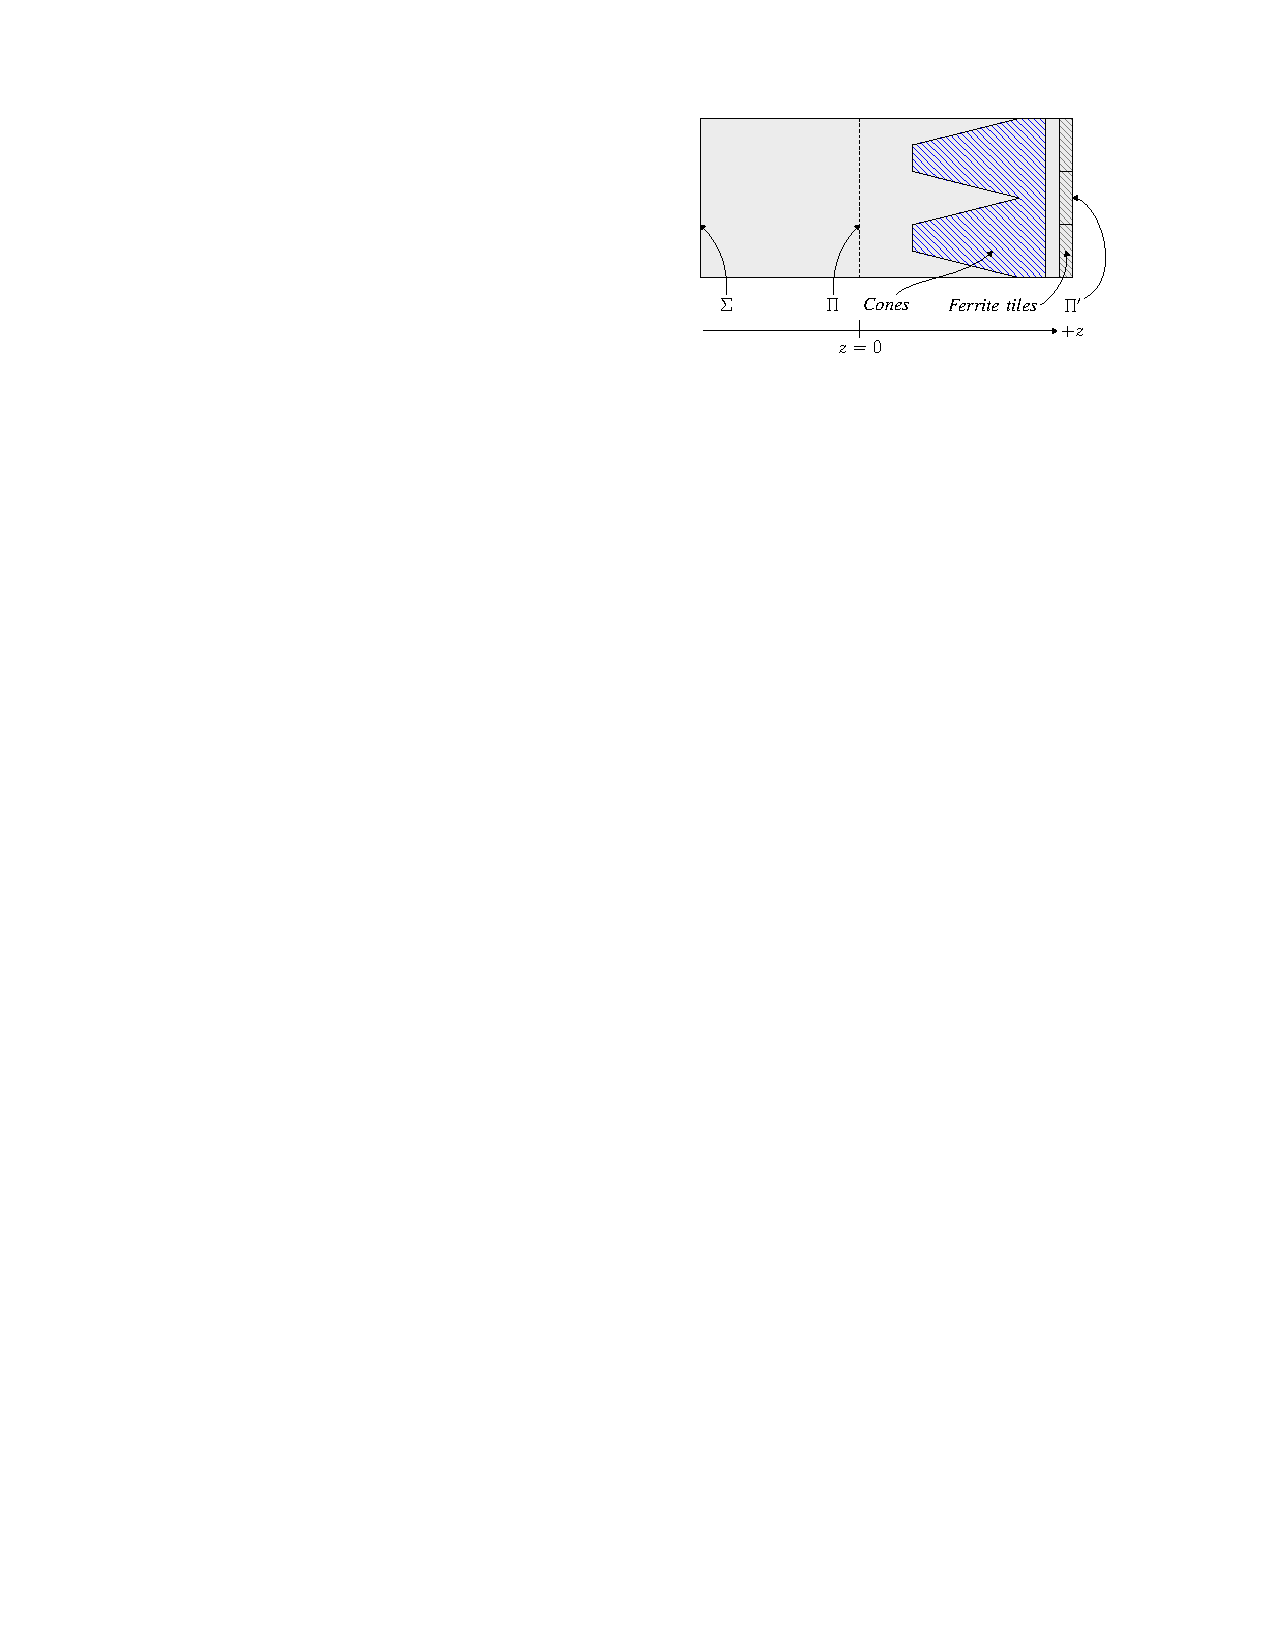
\includegraphics[width=0.9\textwidth]{img/cell_section_poster.pdf}}
            \end{figure}
            \onslide<4->{ \footnotesize   \[
    Z_{\YCalculationPlane'}(z) = Z_c\frac{Z_{\YCalculationPlane} - iZ_c \; tan(\beta z)}{Z_c - iZ_{\YCalculationPlane}\;tan(\beta z)}, \label{eqn:de-embed}
    \]
}
            \begin{figure}
                \onslide<5->{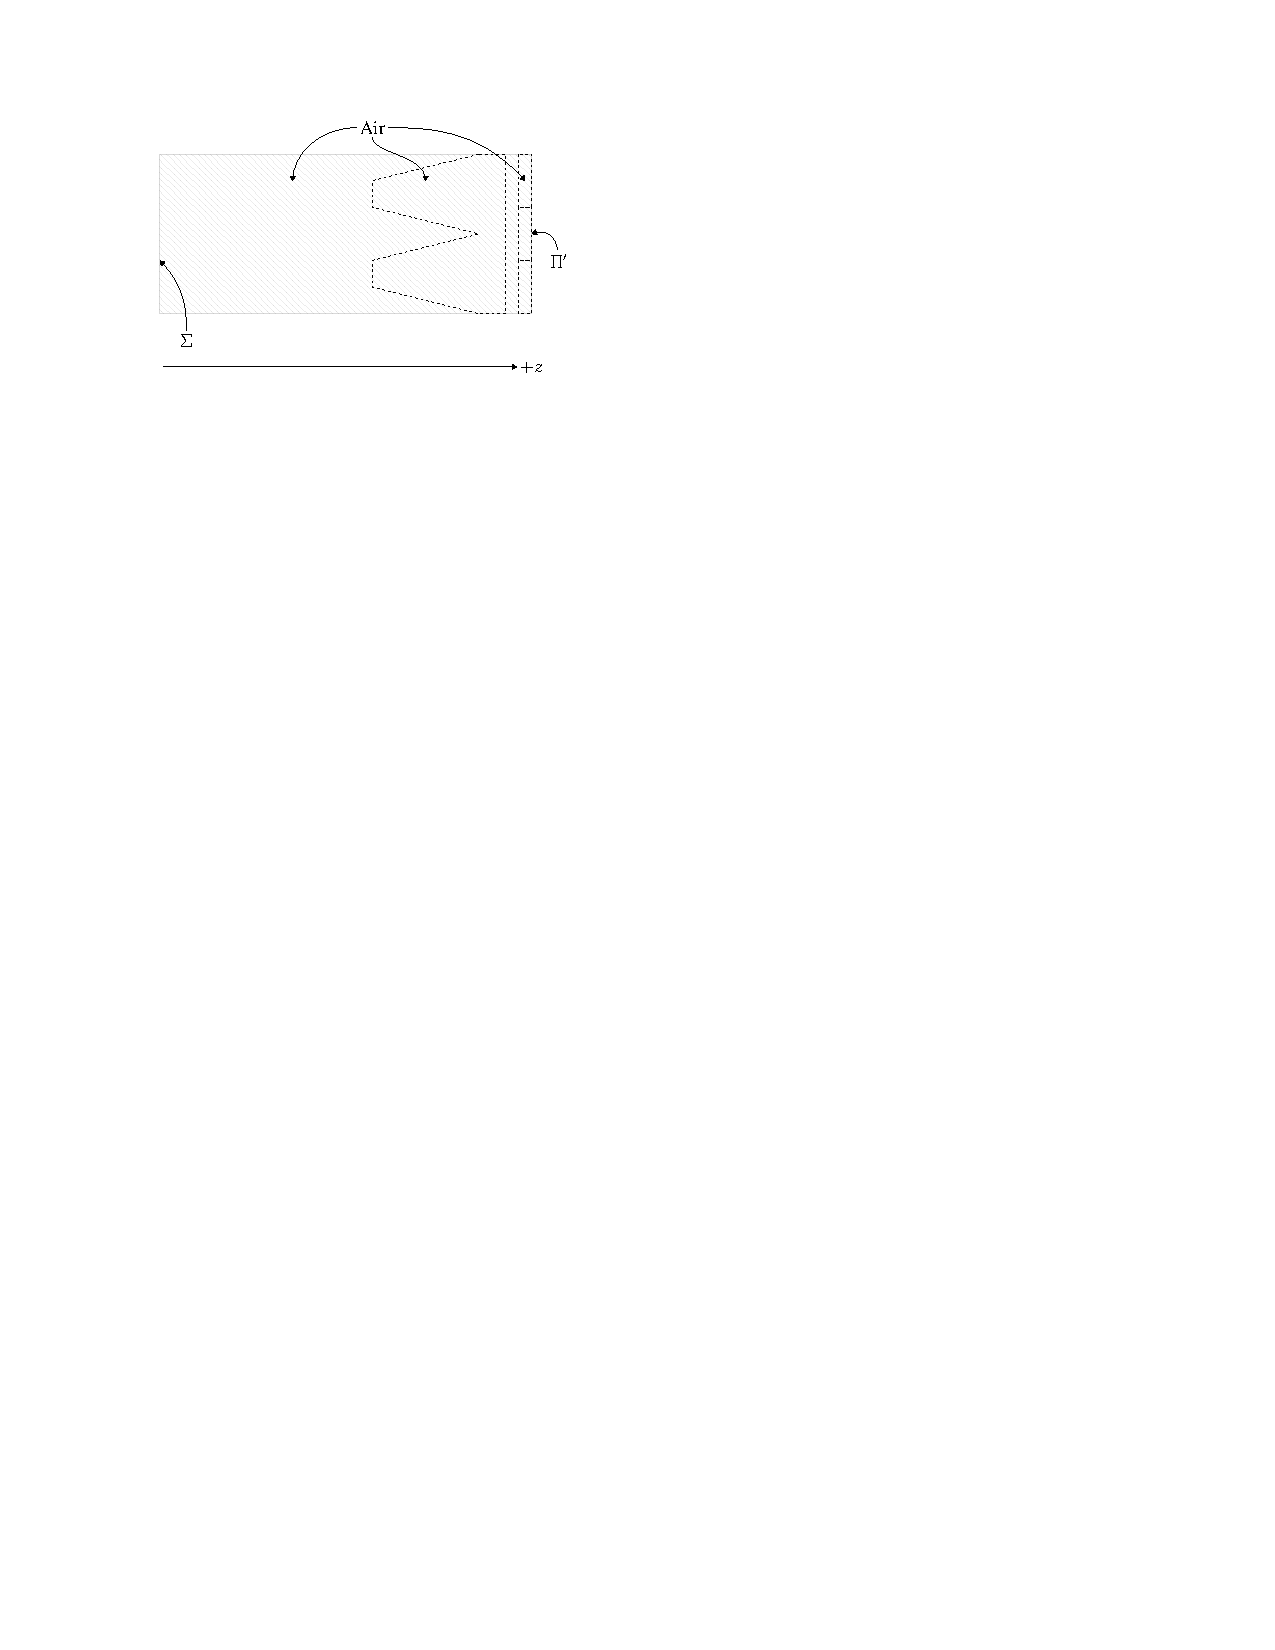
\includegraphics[width=0.9\textwidth]{img/cell_section_equiv_poster.pdf}}
            \end{figure}
        }
        \setbeamercovered{transparent}
    \end{minipage}


    %Modello equivalente: 1/20 elementi, 1/60 tempo di calcolo. Errore nella zona di interesse $< 5$\%.

    %\vspace{5mm}
    %{\small M. Cicuttin, S. Chialina, L. Codecasa, R. Specogna, F. Trevisan \emph{Port boundary conditions for discrete electromagnetic problems in the frequency domain}. Presentato a CEFC2014 e inviato a TMAG.}
    
\end{frame}

%%%%%%%%%%%%%%%%%%%%%%%%%%%%%%%%%%%%%%%%%%%%%%%%%%%%%%%%%%%%%%%%%%%%%%%%%%%%%%%%
\begin{frame}{Equivalent model for anechoic walls: results}
    The proposed equivalent model gave very good results
    \begin{itemize}
        \item it allowed 20x reduction of mesh elements
        %\item it allowed 60x reduction of computation times
        \item in the whole area of interest the relative error was below 5\%
    \end{itemize}

    \begin{figure}
        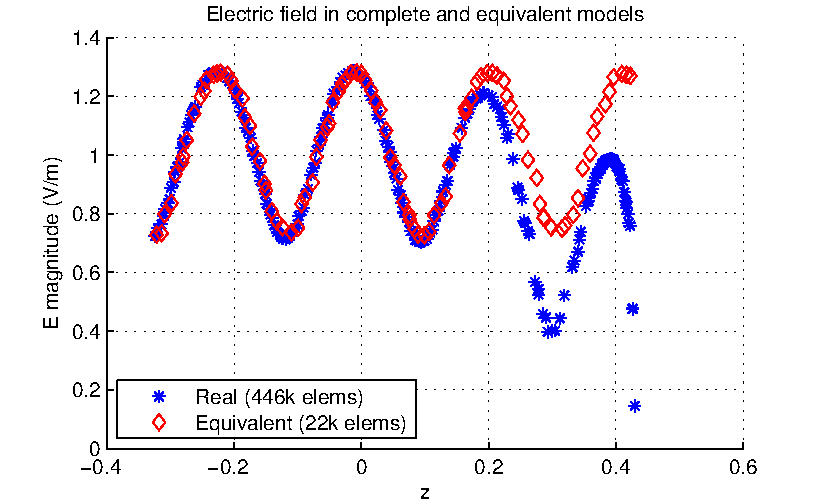
\includegraphics[width=0.5\textwidth]{img/efield_cmp_2.pdf}
        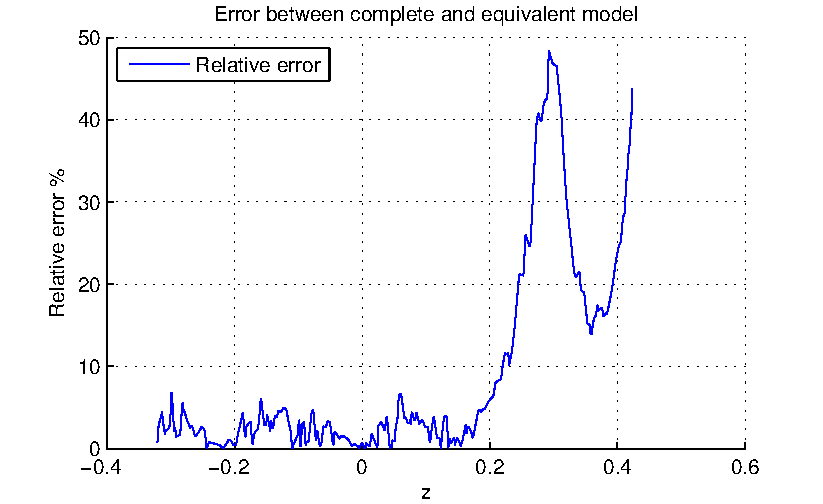
\includegraphics[width=0.5\textwidth]{img/error_2.pdf}
    \end{figure}
    
\end{frame}

%%%%%%%%%%%%%%%%%%%%%%%%%%%%%%%%%%%%%%%%%%%%%%%%%%%%%%%%%%%%%%%%%%%%%%%%%%%%%%%%
\begin{frame}[fragile]{Equivalent radiating elements}
    We would like to have a simple object (a sphere) that radiates a field equivalent to the one that is radiated by a more complex antenna
    \pause
    \begin{itemize}
        \item Simulate the real antenna with NEC/HFSS/FEKO
        \item Calculate the field on the reference sphere
        \item Insert the sphere (that radiates the calculated field) in the simulation environment
    \end{itemize}
    
    \pause
    \begin{minipage}{0.59\textwidth}
        Two regions:
        \begin{itemize}
            \item Total field
            \item Scattering field
        \end{itemize}
        The formulation allows to evaluate (inside the sphere) only the ``reaction'' of the environment.
    \end{minipage}
    \hspace{1cm}
    \scalebox{0.4}{
        \begin{minipage}{0.39\textwidth}
            \begin{figure}
                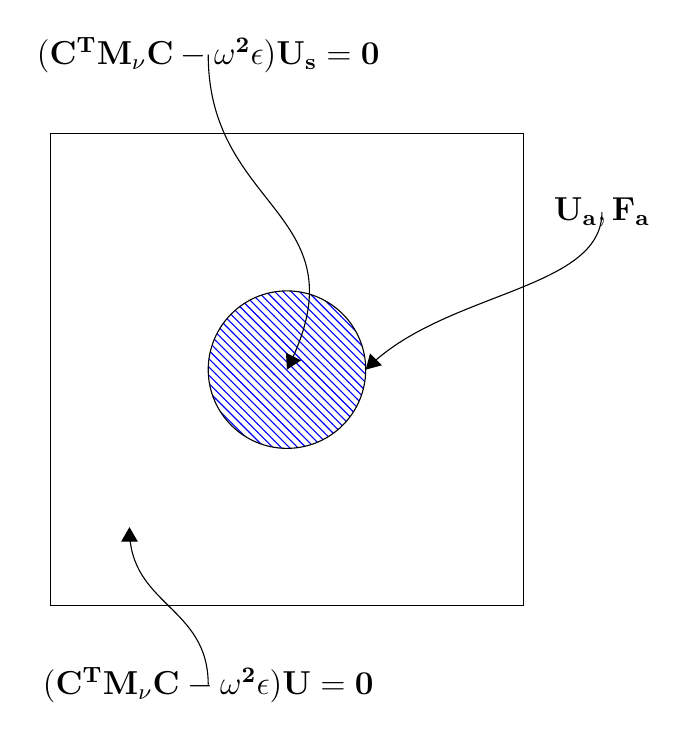
\begin{tikzpicture}
                    \draw [pattern=north west lines, pattern color=blue] (0,0) ellipse (1 and 1);
                    \draw  (-3,3) rectangle (3,-3);
                    \node (v1) at (-1,-4) {\large $(\mathbf{C^TM_{\nu}C - \omega^2\epsilon)U=0}$};
                    \draw [-triangle 60](-1,-4) .. controls (-1,-3) and (-2,-3) .. (-2,-2);
                    \draw [-triangle 60](-1,4) .. controls (-1,2) and (1,2) .. (0,0);
                    \node at (-1,4) {\large $(\mathbf{C^TM_{\nu}C - \omega^2\epsilon)U_s=0}$};
                    \node at (4,2) {\large$\mathbf{U_a},\mathbf{F_a}$};
                    \draw [-triangle 60](4,2) .. controls (4,1) and (2,1) .. (1,0);
                \end{tikzpicture}
            \end{figure}
    \end{minipage}
    }
\end{frame}


%%%%%%%%%%%%%%%%%%%%%%%%%%%%%%%%%%%%%%%%%%%%%%%%%%%%%%%%%%%%%%%%%%%%%%%%%%%%%%%%
\begin{frame}{Validation}
    \small
    The code was validated against
    \begin{itemize}
        \item analytical solution of simple problems
        \item other codes
        \item \textcolor{uniud-orange}{real-world meausurements} (not trivial!)
    \end{itemize}
    \pause
    I made the measurements in the anechoic rooms of Emilab SRL, an EMC laboratory. Two experiments were of particular significance:
    \vspace{2mm}

    \begin{minipage}{0.5\textwidth}
        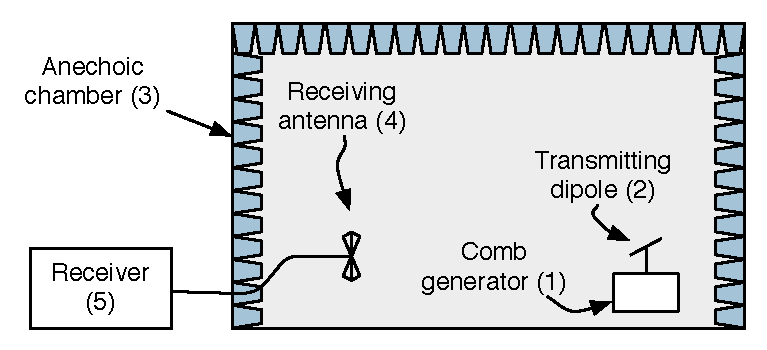
\includegraphics[width=\textwidth]{img/setup.pdf}

        {\tiny CE room, 558 comparison points}
    \end{minipage}
    \hfill
    \begin{minipage}{0.4\textwidth}
        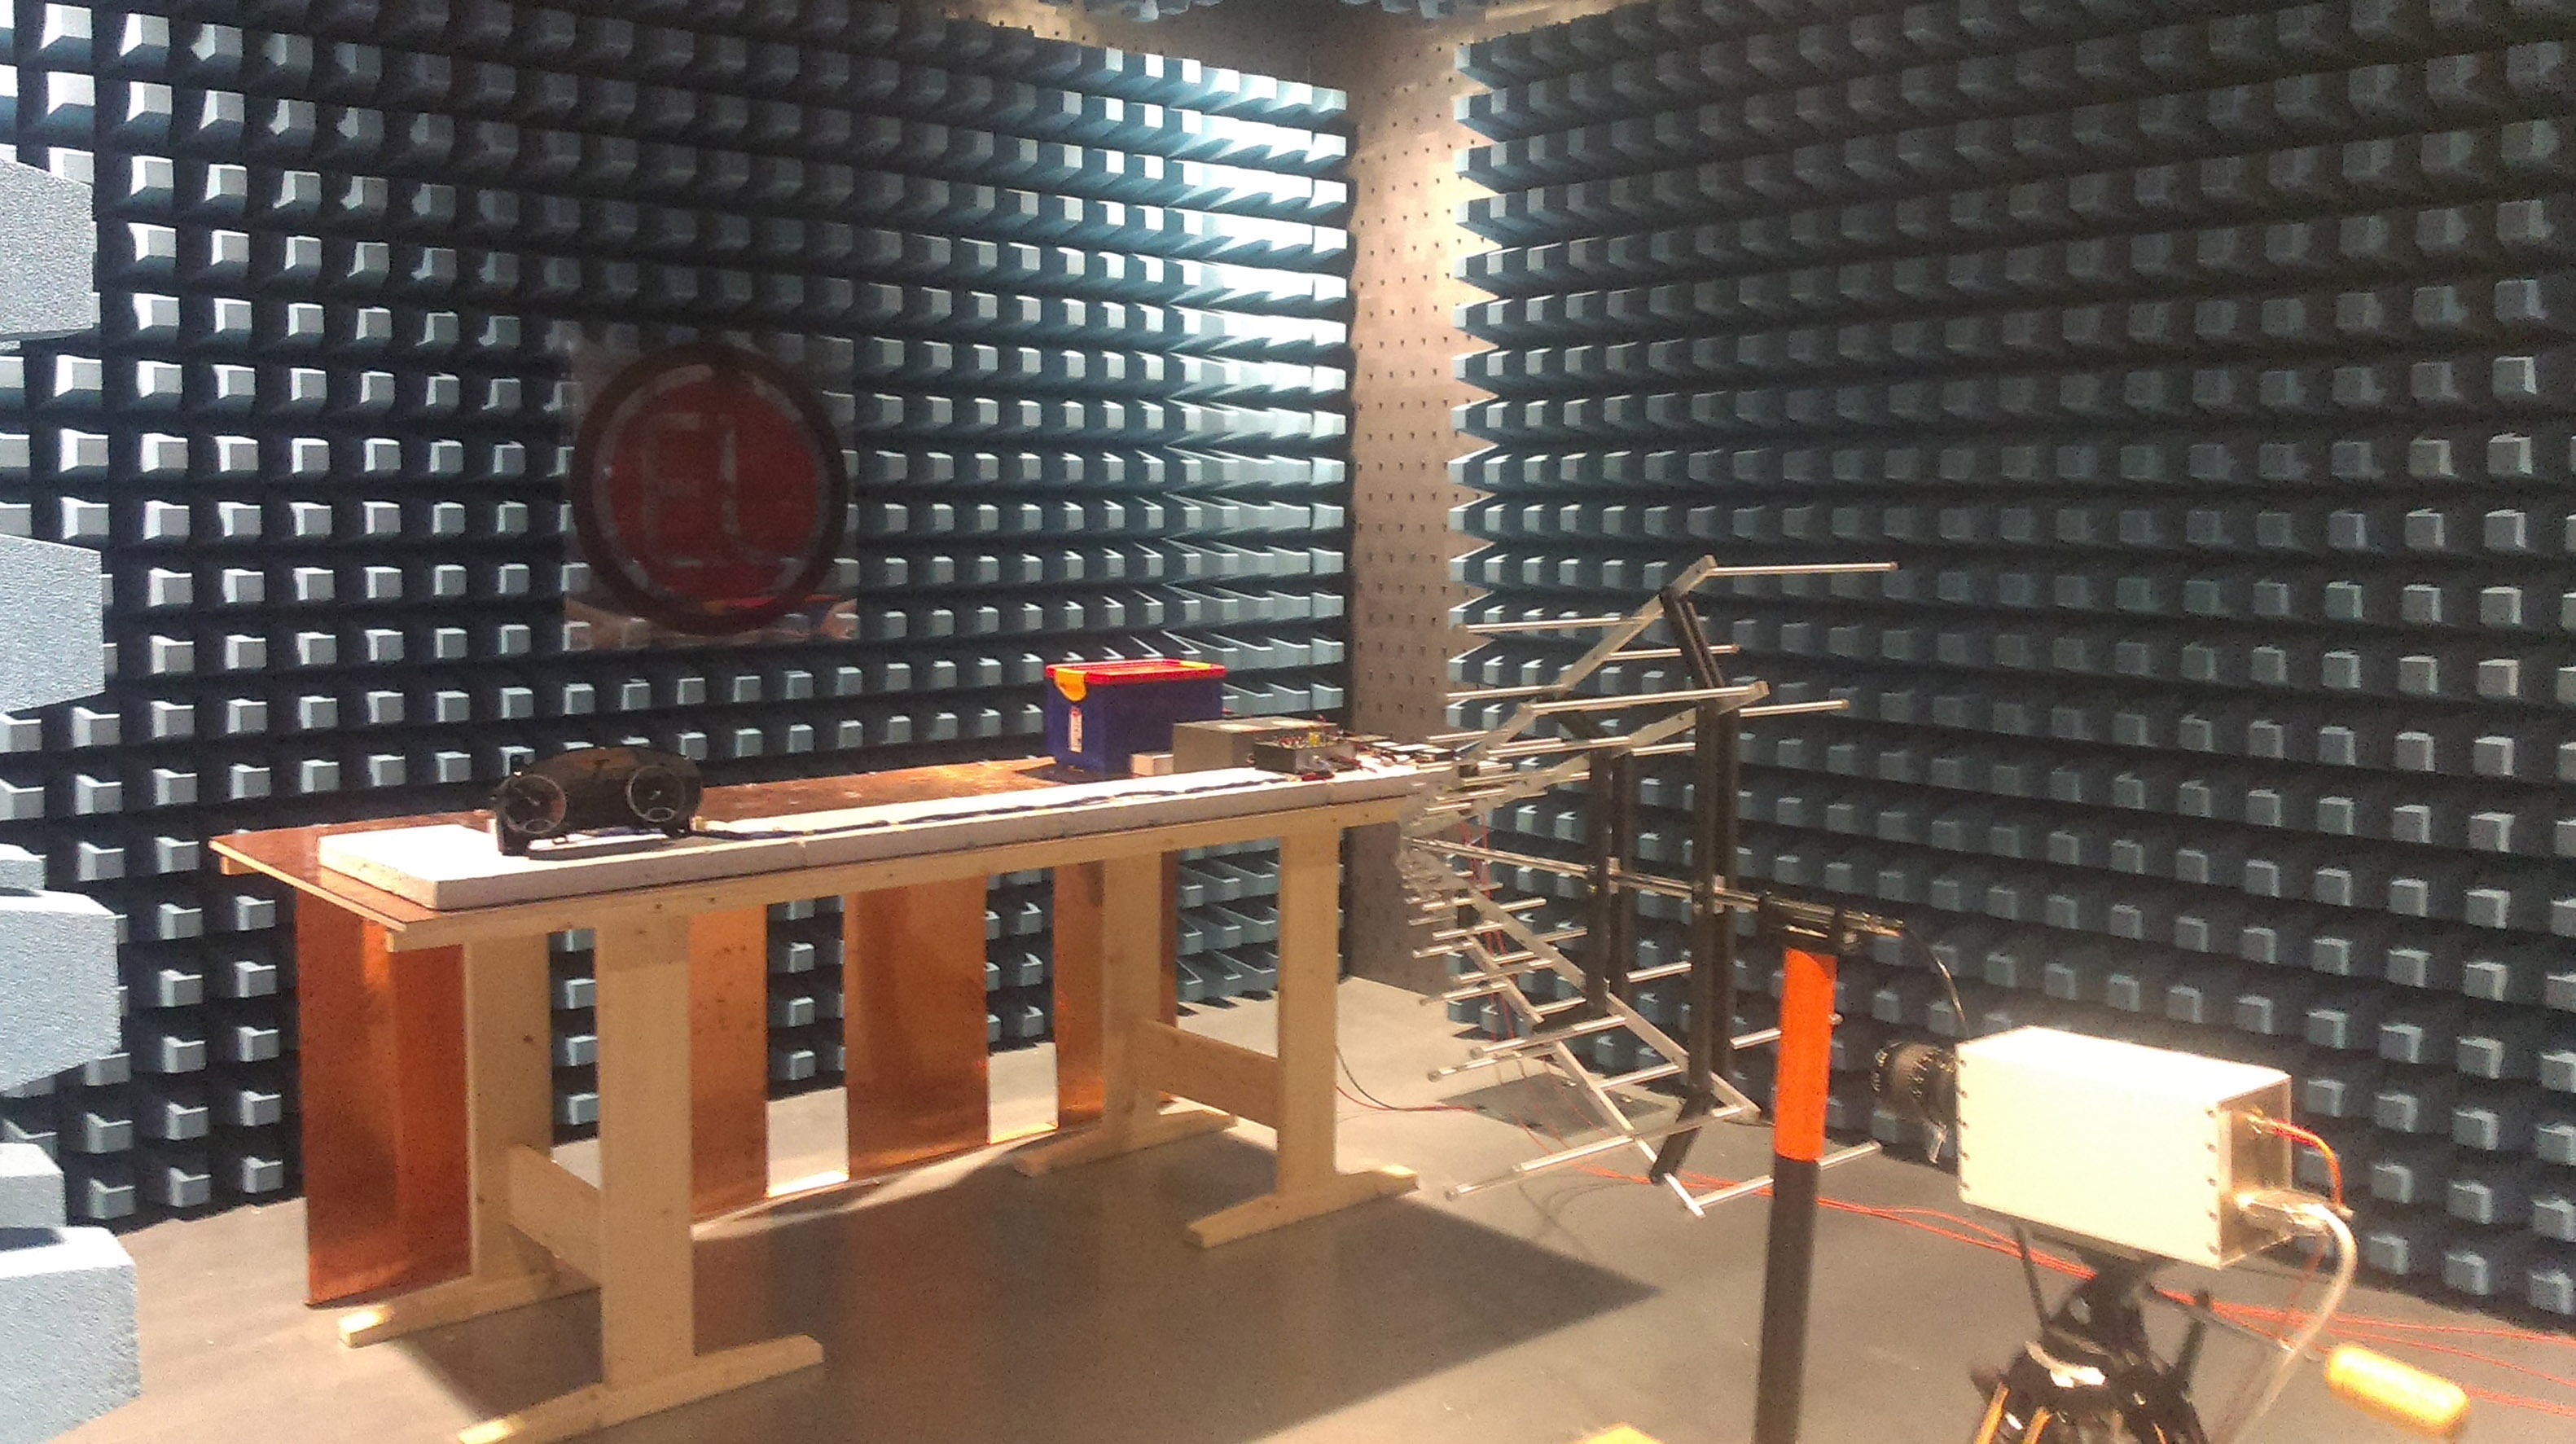
\includegraphics[width=\textwidth]{img/camera.jpg}

        {\tiny Automotive room, 30 comparison points}
    \end{minipage}%

    \vspace{2mm}

    \textcolor{uniud-orange}{Idea: site-to-site comparison as mandated by ISO 17025:2005, not between real sites but between a real site and a \emph{virtual site}.}
\end{frame}

%%%%%%%%%%%%%%%%%%%%%%%%%%%%%%%%%%%%%%%%%%%%%%%%%%%%%%%%%%%%%%%%%%%%%%%%%%%%%%%%
\begin{frame}{CE room experiment: description}
    \footnotesize
    %\begin{itemize}
    %    \item Radiating object placed in an anechoic room 
    %    \item Generated field measured at specific points
    %    \item Measurements compared with simulations
    %    \end{itemize}
    %\vfill

    \begin{minipage}{0.48\textwidth}
        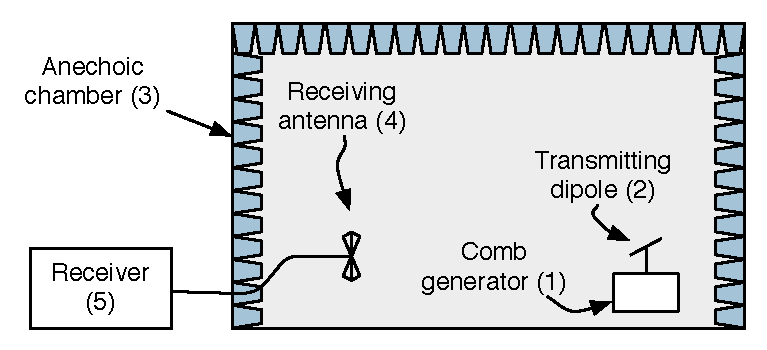
\includegraphics[width=\textwidth]{img/setup.pdf}

        Some preliminary steps required:
        \begin{itemize}
            \item Comb generator characterization
            \item TX antenna characterization
            \item Antenna current measurement
            %\item Actual E-field measurements
        \end{itemize}
    \end{minipage}
    \hfill
    \begin{minipage}{0.48\textwidth}
        About the setup:
        \begin{itemize}
            \item RX at $h = {1m, 1.5m, 2m}$
            \item TX at $h = {1m, 1.5m, 2m}$
            \item Horizontal and vertical polarizations
            \item From 90 to 390 MHz at 10 MHz steps
        \end{itemize}
        A total of 558 comparison points!
    \end{minipage}
    \vfill

    Large discrepancies initially found on some points: we used an imperfect setup. 
    
    \textcolor{uniud-orange}{Simulation allowed to discover measurement problems!}

\end{frame}

%%%%%%%%%%%%%%%%%%%%%%%%%%%%%%%%%%%%%%%%%%%%%%%%%%%%%%%%%%%%%%%%%%%%%%%%%%%%%%%%
\begin{frame}{CE room experiment: results}
    \footnotesize
    \begin{minipage}{0.48\textwidth}
        TX and RX @ 1m, horizontal

        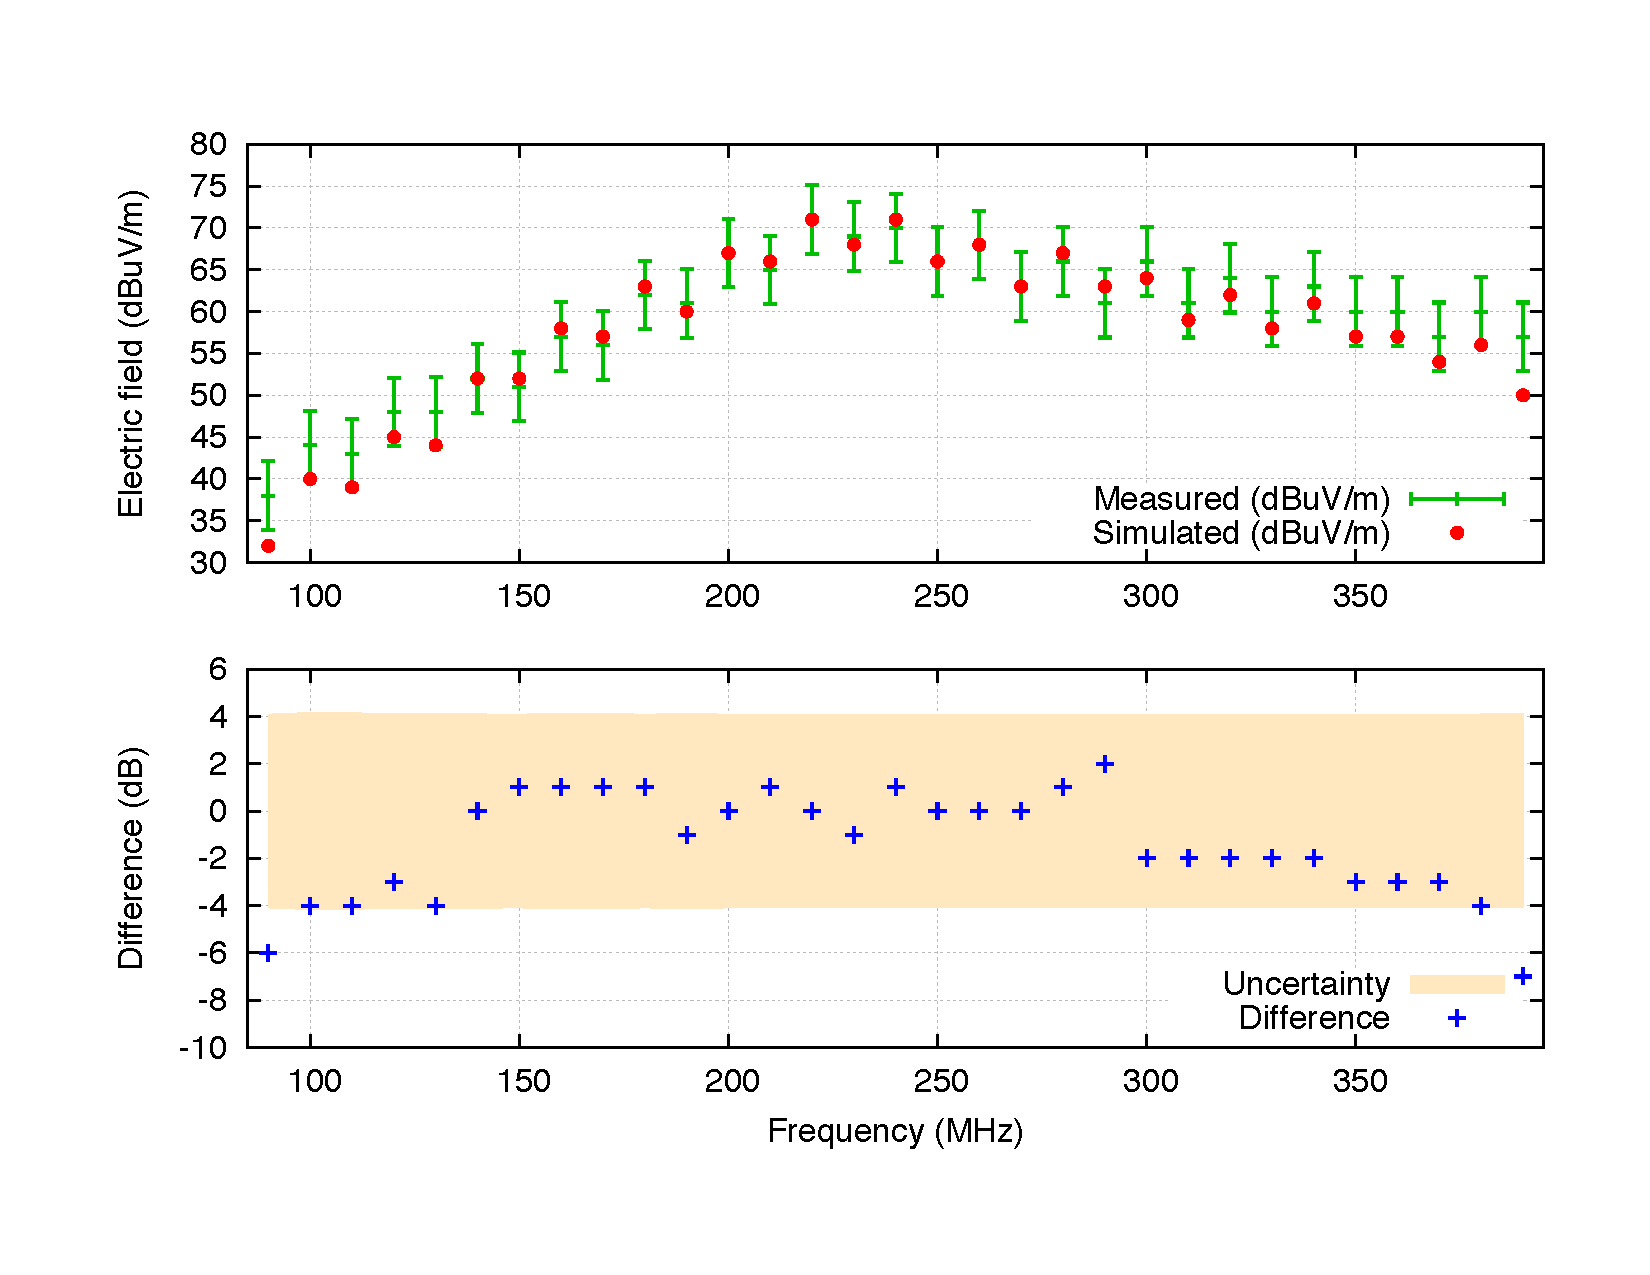
\includegraphics[width=0.8\textwidth]{img/comparison100h.pdf}

        \vspace{4mm}
        TX and RX @ 1.5m, vertical

        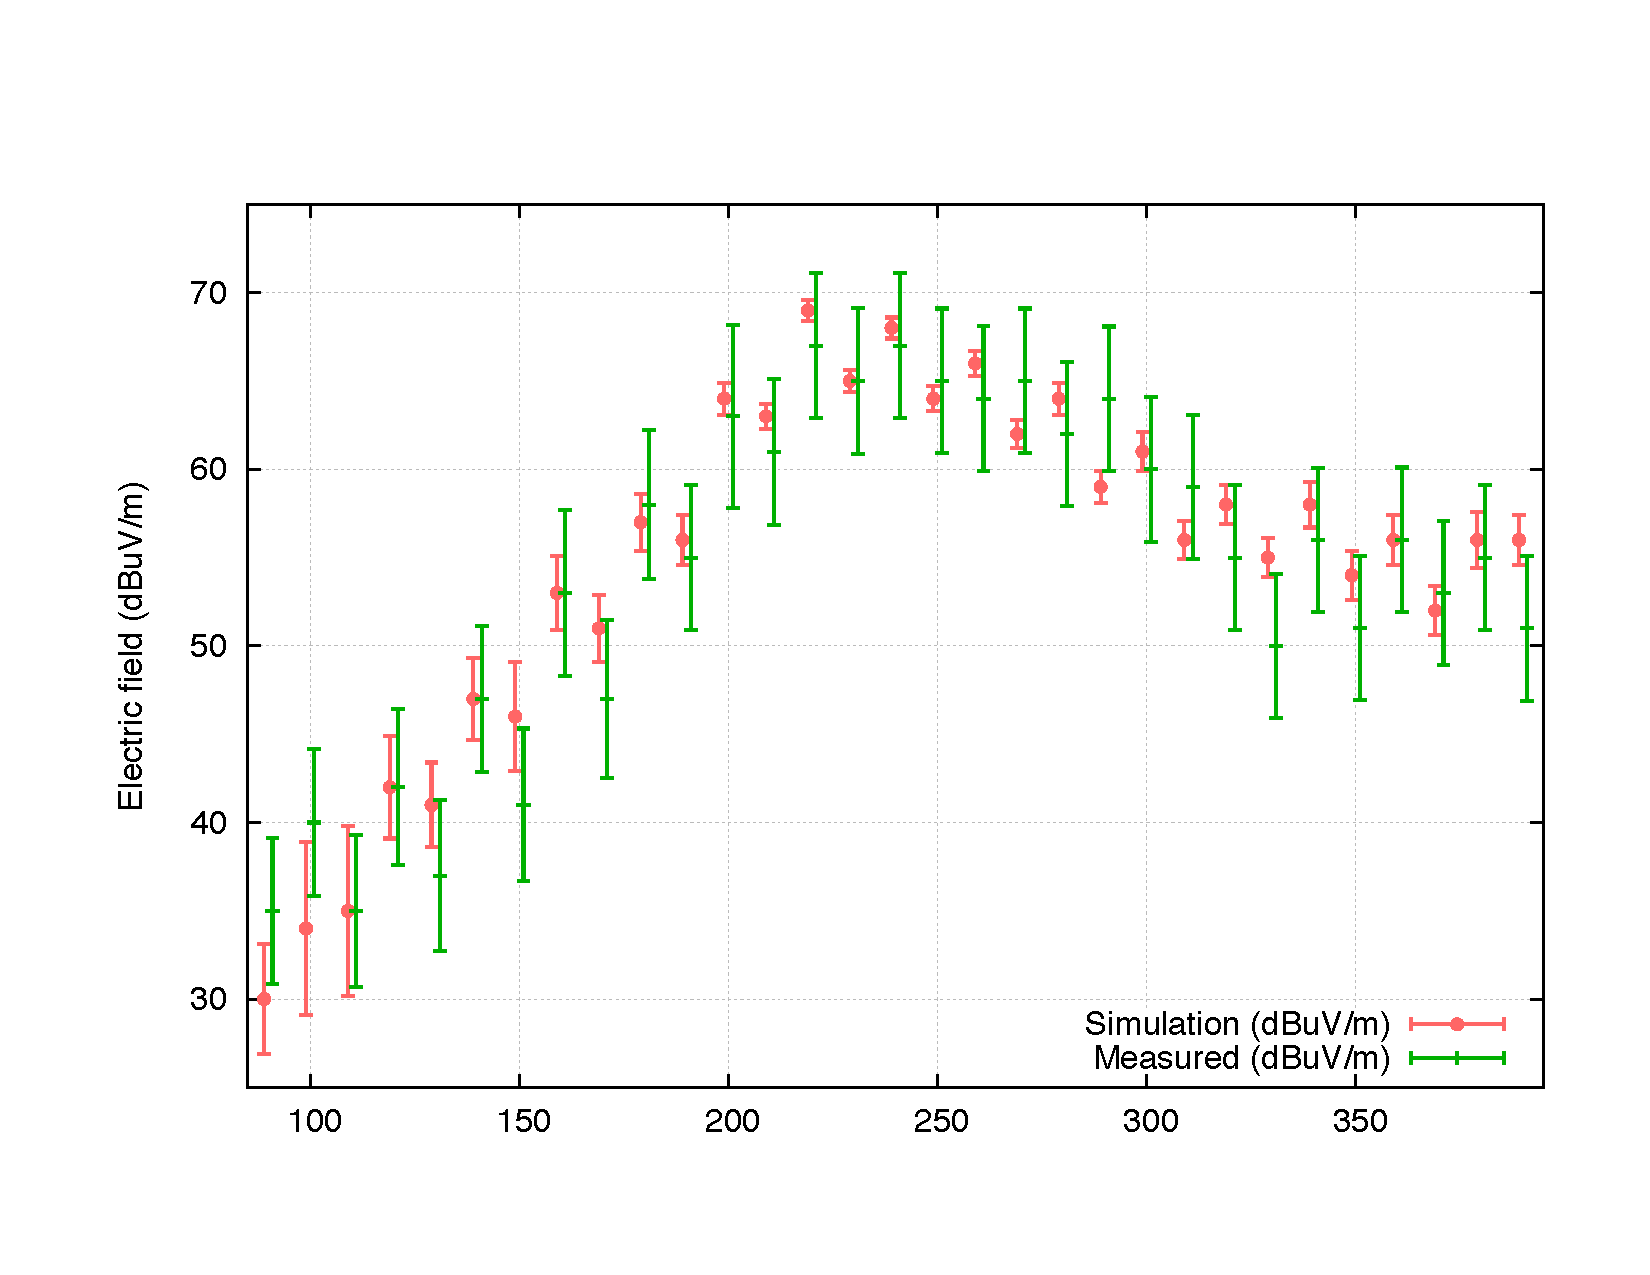
\includegraphics[width=0.8\textwidth]{img/comparison150v.pdf}

    \end{minipage}
    \hfill
    \begin{minipage}{0.48\textwidth}
        TX @ 1m horizontal, 230 MHz

        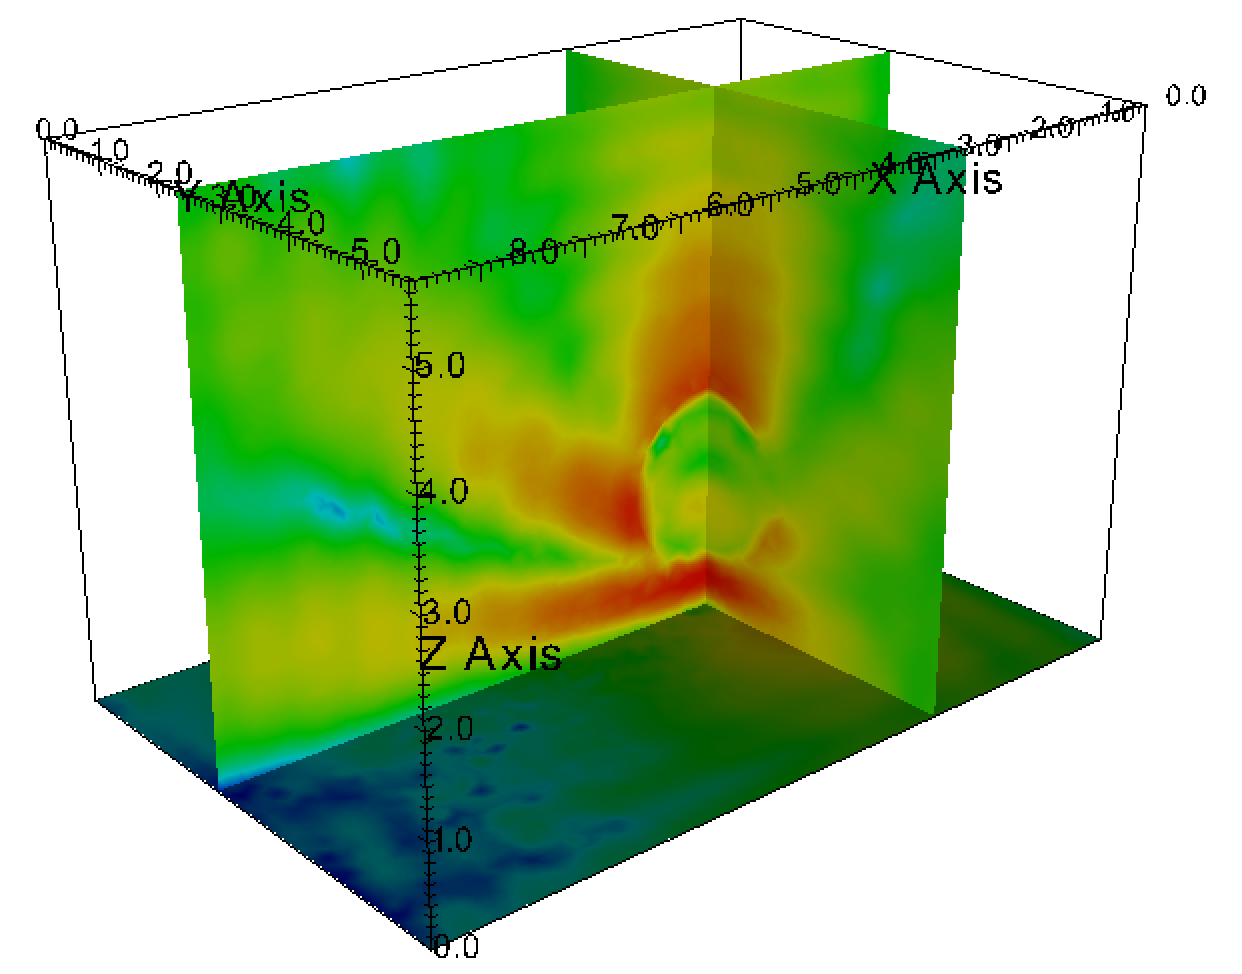
\includegraphics[width=0.8\textwidth]{img/ant230}

        RX @ 1m, 1.5m and 2m

        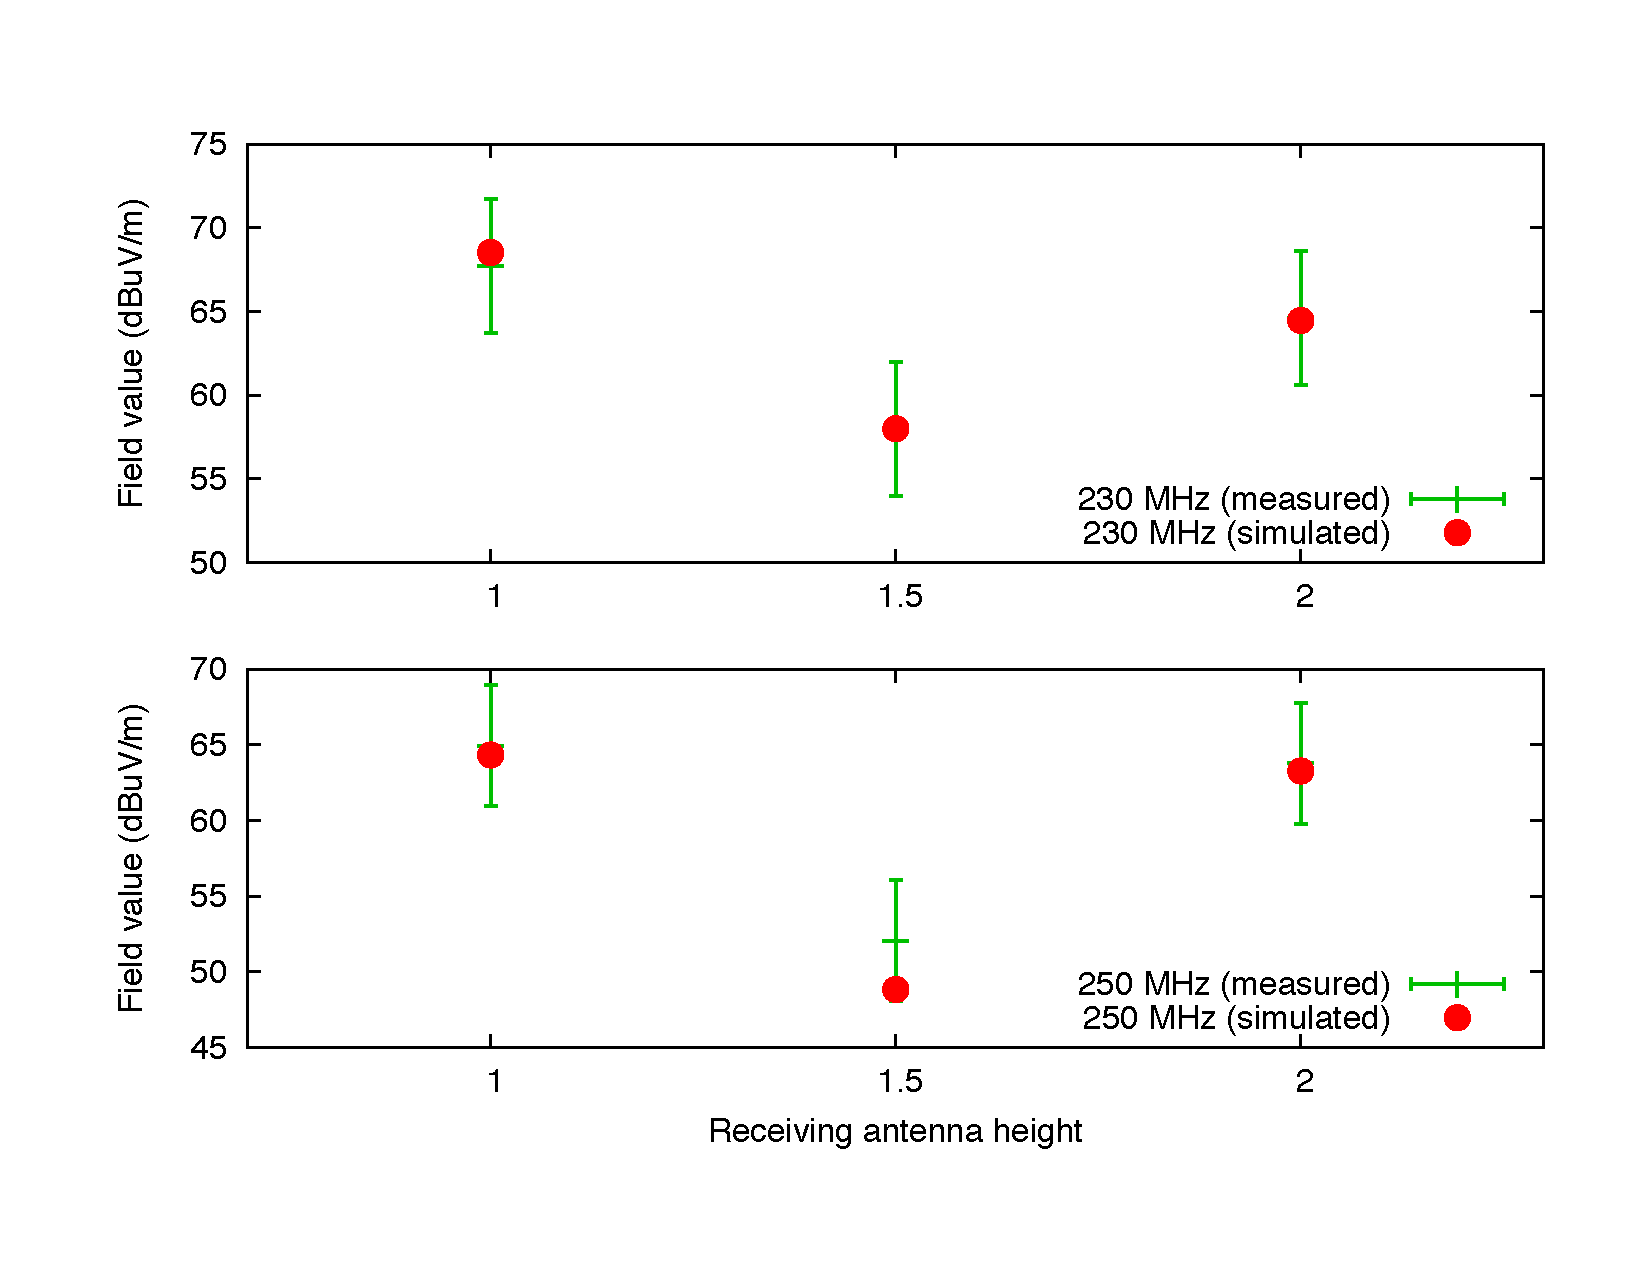
\includegraphics[width=0.8\textwidth]{img/hole}
    \end{minipage}
\end{frame}

%%%%%%%%%%%%%%%%%%%%%%%%%%%%%%%%%%%%%%%%%%%%%%%%%%%%%%%%%%%%%%%%%%%%%%%%%%%%%%%%
\begin{frame}{Automotive room experiment: description}
    \footnotesize
    Automotive test compliant table inside the room. Aim: evaluate its effect. 
    \vspace{3mm}

    Experimental procedure almost equal as the previous one.
    \vspace{3mm}

    Used a small dipole as receiving antenna $\implies$ required careful characterization.

    \begin{figure}
        \centering
        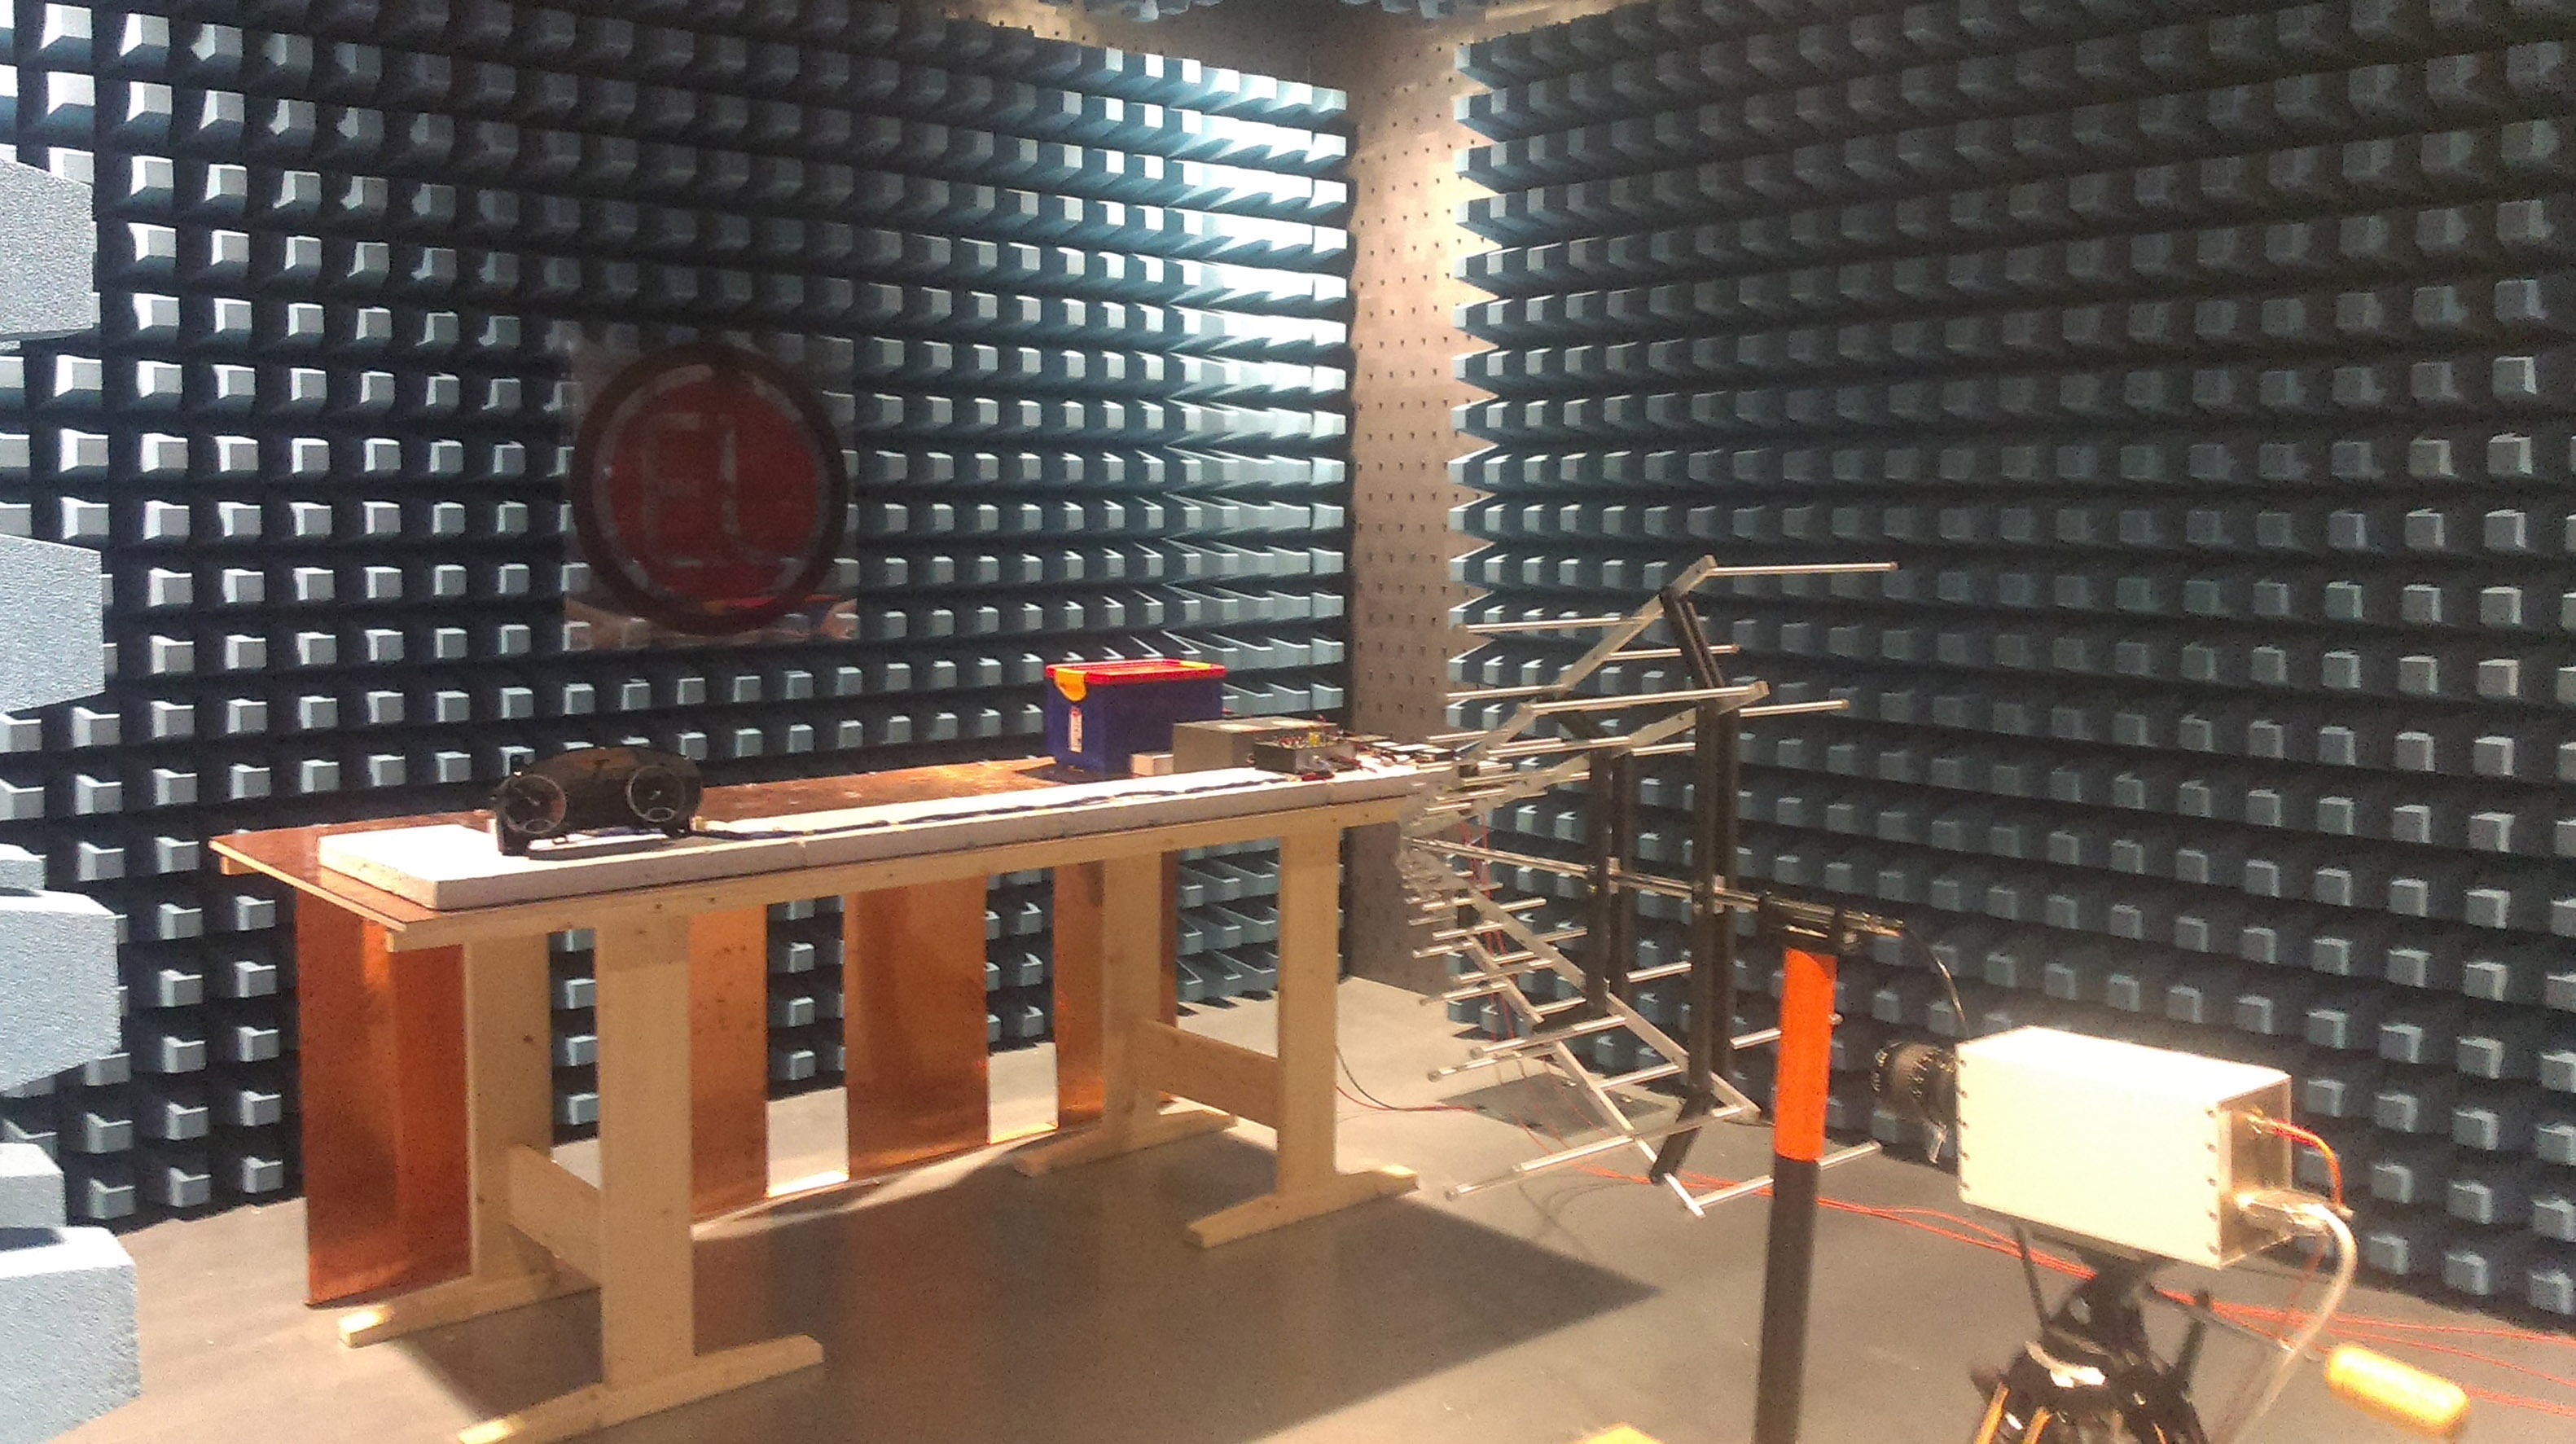
\includegraphics[width=0.5\textwidth]{img/camera.jpg}
    \end{figure}
    A transmitting dipole was placed at 1 meter in front of the table, in horizontal polarization. 
\end{frame}
%%%%%%%%%%%%%%%%%%%%%%%%%%%%%%%%%%%%%%%%%%%%%%%%%%%%%%%%%%%%%%%%%%%%%%%%%%%%%%%%
\begin{frame}{Automotive room experiment: results}
    \footnotesize
    \begin{minipage}{0.48\textwidth}
        Unexpected standing wave under the table predicted by simulation:  measurements confirmed its presence!

        \vspace{5mm}

    Automotive room is very busy, time for only 30 measurements.

    \vspace{5mm}

    Precise measurements in this setup were rather difficult.

    \end{minipage}
    \hfill
    \begin{minipage}{0.48\textwidth}

        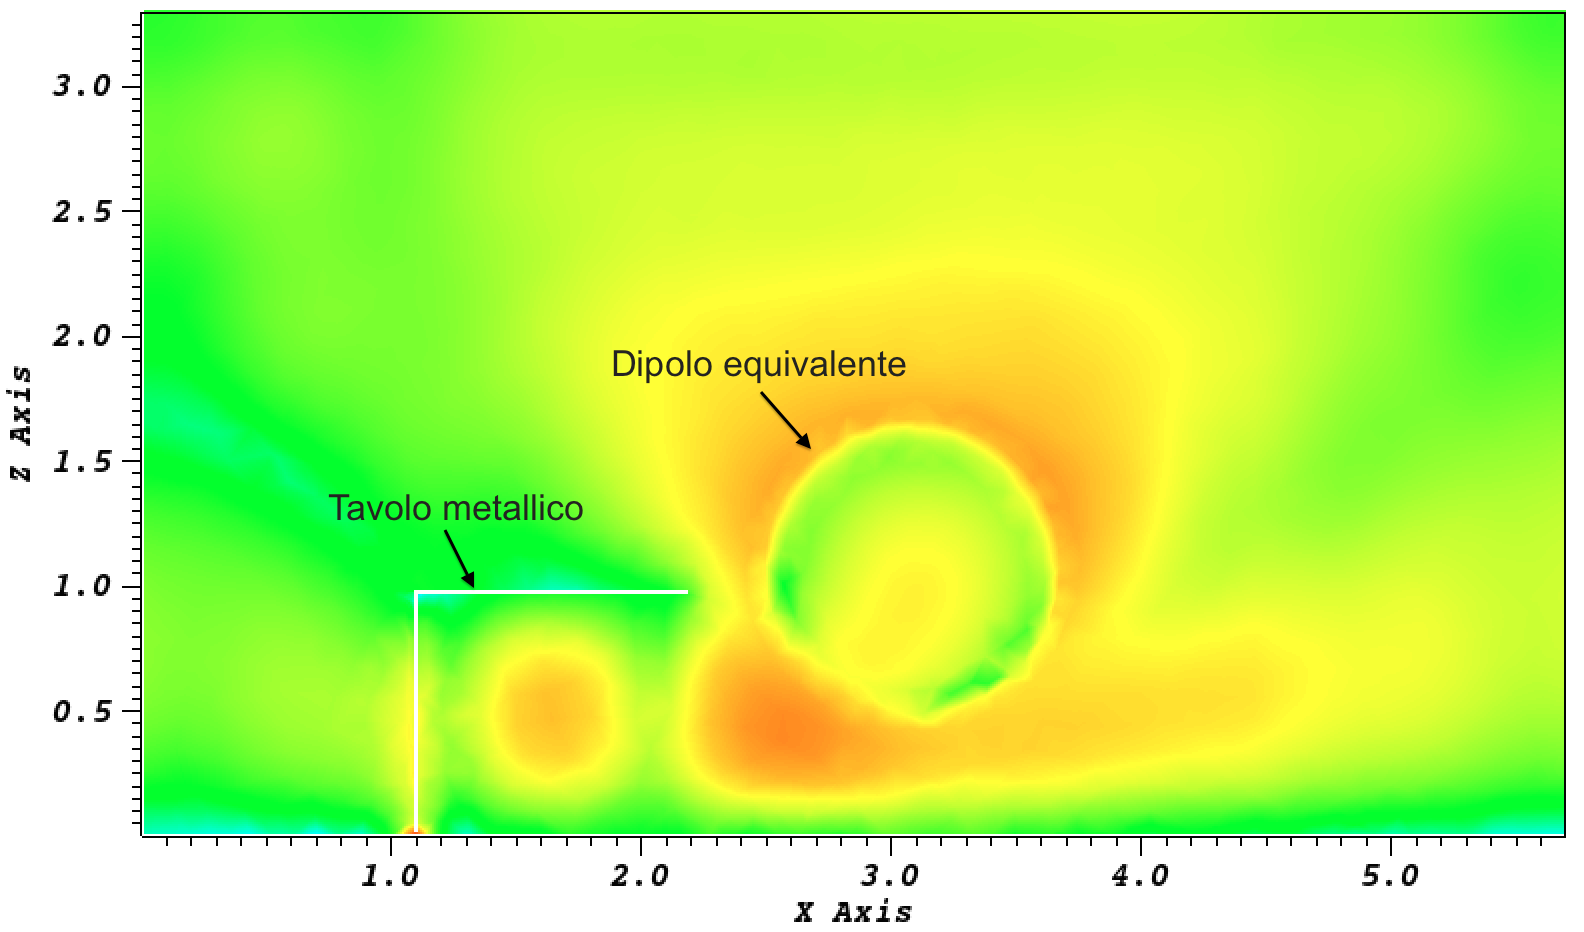
\includegraphics[width=0.8\textwidth]{img/camera_alse}

        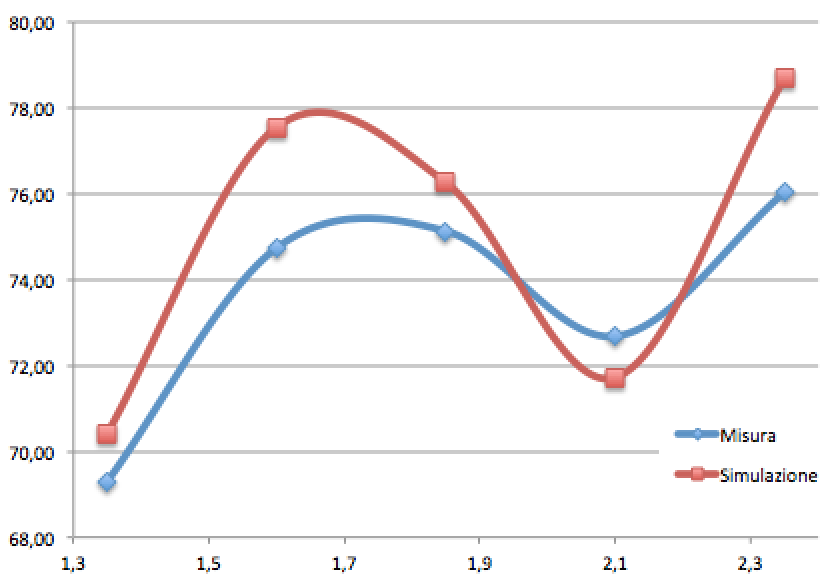
\includegraphics[width=0.8\textwidth]{img/campo_alse}

    \end{minipage}

    \vspace{5mm}

    \textcolor{uniud-orange}{There is \textbf{a lot} more to say about the experiments, especially about the equipment characterization and the criticalities of these measurements. If interested please ask during poster session!}

\end{frame}

%%%%%%%%%%%%%%%%%%%%%%%%%%%%%%%%%%%%%%%%%%%%%%%%%%%%%%%%%%%%%%%%%%%%%%%%%%%%%%%%
\begin{frame}{Complementarity and adaptive mesh refinement}
    Frequency domain wave propagation can be described mathematically in two ways
    \vspace{5mm}

    \pause
    \begin{minipage}{0.48\textwidth}
        \begin{center}
        \underline{the E-formulation}

        $\nabla\times\mu^{-1}\nabla\times\mathbf{E} - \omega^2\epsilon\mathbf{E} = 0$

        $\Downarrow$

        $\mathbf{C}^T\mathbf{M}_{\mu^{-1}}\mathbf{CU} - \omega^2\mathbf{M}_{\epsilon}\mathbf{U} = 0$
    \end{center}

    \end{minipage}
    \pause
    \begin{minipage}{0.48\textwidth}
        \begin{center}
        \underline{the H-formulation}

        $\nabla\times\epsilon^{-1}\nabla\times\mathbf{H} - \omega^2\mu\mathbf{H} = 0$

        $\Downarrow$

        $\mathbf{C}^T\mathbf{M}_{\epsilon^{-1}}\mathbf{CF} - \omega^2\mathbf{M}_{\mu}\mathbf{F} = 0$
    \end{center}

    \end{minipage}

    \pause
    \vspace{5mm}

    \begin{minipage}{0.60\textwidth}
        \begin{itemize}
            \item Continuous formulations are equivalent, discrete ones are not!
            \item Comparing the differences error can be estimated and adaptive refinement can be done.
            \item Why? Adaptivity reduces number of elements further.
            \end{itemize}
    \end{minipage}
    \hfill
    \begin{minipage}{0.25\textwidth}
    \begin{figure}
        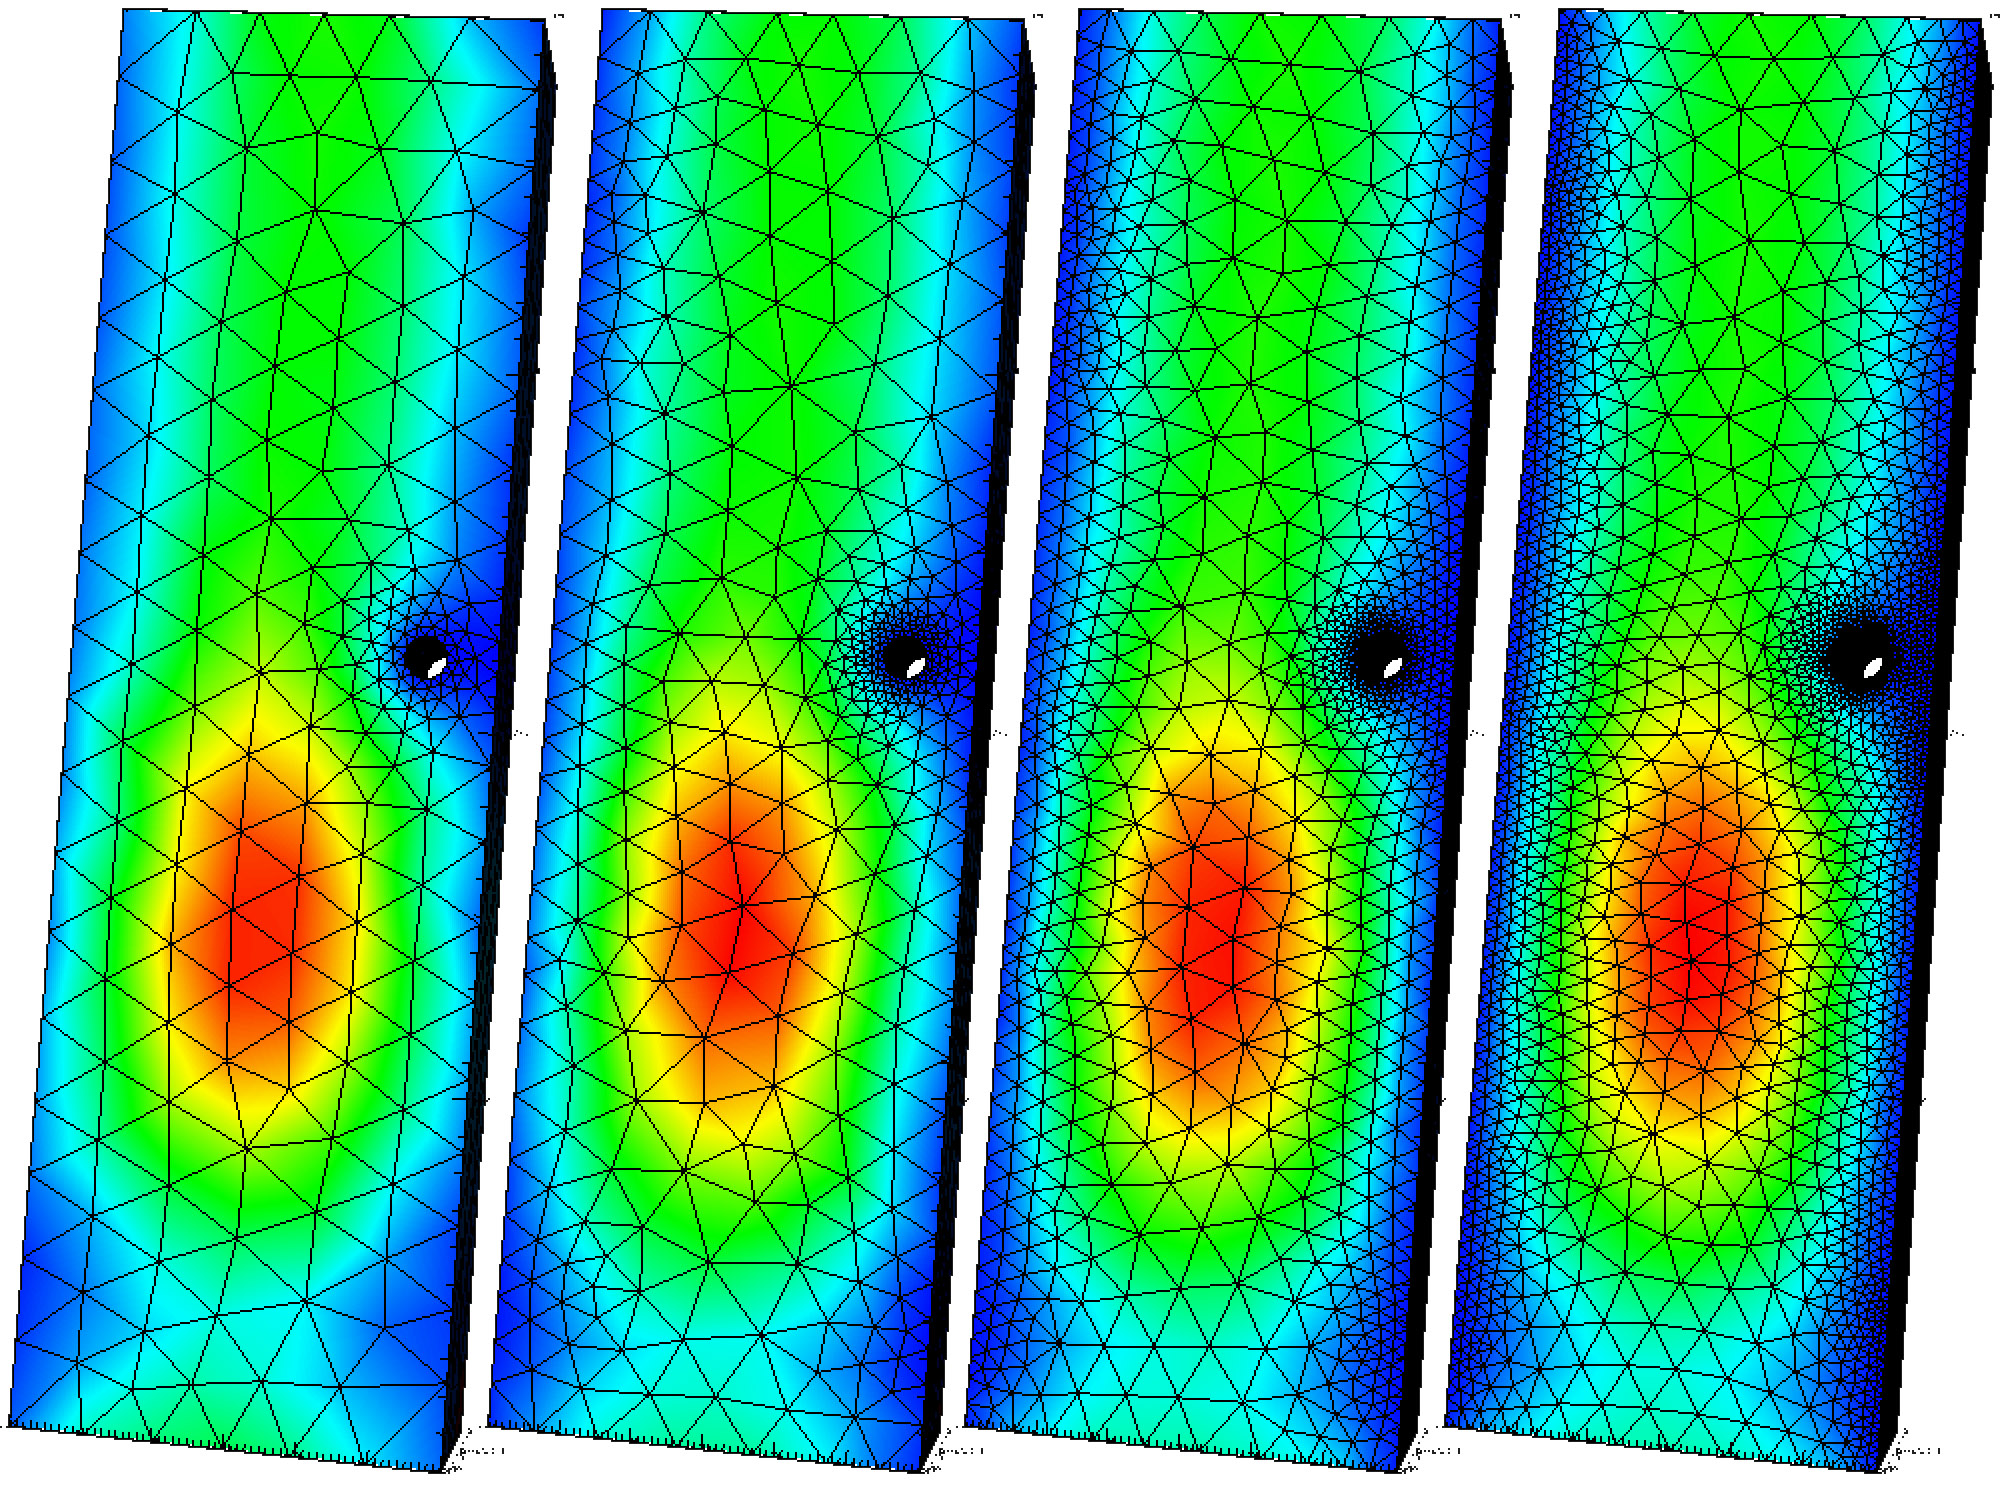
\includegraphics[width=\textwidth]{img/refinement.jpg}
    \end{figure}
\end{minipage}
\hfill


\end{frame}

%%%%%%%%%%%%%%%%%%%%%%%%%%%%%%%%%%%%%%%%%%%%%%%%%%%%%%%%%%%%%%%%%%%%%%%%%%%%%%%%
\begin{frame}{$A-\chi$ formulation and field-circuit coupling}
    \small
    Aim: separate $\mathbf{E}$ in rotational and irrotational parts ($\mathbf{E} = -\nabla\phi - i\omega\mathbf{A})$. Propagation written in terms of vector potential $\mathbf{A}$ and scalar potential $\chi$.

    \begin{center}
        ($\mathbf{C}^T\mathbf{M}_{\mu^{-1}}\mathbf{C} + i\omega\mathbf{Y} - \omega^2\mathbf{M}_{\epsilon} + i\omega\mathbf{M}_{\sigma})(\mathbf{A} + \mathbf{G\chi}) = \mathbf{I_s} + 2\mathbf{F^{b^-}}$
    \end{center}
    
    No time for the details, but I'm available during poster session! However:
    \begin{itemize}
        \item it will allow field-circuit coupling
        \item ``field'' part of the code already in place, minor things to fix
    \end{itemize}

    \vfill
    Could allow to study disturbances due to external RF fields to the operation of the device under test.

\end{frame}

%%%%%%%%%%%%%%%%%%%%%%%%%%%%%%%%%%%%%%%%%%%%%%%%%%%%
\begin{frame}{Publications}

    {\footnotesize \underline{Journal papers:}}

    \begin{itemize}
        \item {\scriptsize S. Chialina, M. Cicuttin, L. Codecasa, R. Specogna, and F. Trevisan, ``\emph{Plane Wave Excitation for Frequency Domain Electromagnetic Problems by Means of Impedance Boundary Condition}'', IEEE Trans. Magn., vol. 51, no. 3, 2015.}
        \item {\scriptsize S. Chialina, M. Cicuttin, L. Codecasa, G. Solari, R. Specogna, and F. Trevisan, ``\emph{Modeling of anechoich chambers with equivalent materials and equivalent sources}'', Accepted by IEEE Trans. EMC}
    \end{itemize}

    {\footnotesize \underline{Papers accepted at COMPUMAG 2015 (and submitted to IEEE TMAG):}}
    \begin{itemize}
        \item {\scriptsize MC, LC, RS, and FT, ``\emph{Complementary discrete geometric h-field formulation for wave propagation problems}'' [\textcolor{red}{oral presentation}, 5\% of the accepted papers]}

        \item {\scriptsize MC, L. Codecasa, R. Specogna, and F. Trevisan, ``\emph{Excitation by scattering/total field decomposition and UPML in the geometric formulation}'' [poster]}

        \item {\scriptsize A. Affanni, MC, R. Specogna, and F. Trevisan, ``\emph{Fast uncertainty quantification of fields and global quantities}'' [poster]}

    \end{itemize}

\end{frame}


%%%%%%%%%%%%%%%%%%%%%%%%%%%%%%%%%%%%%%%%%%%%%%%%%%%%
\begin{frame}{Thesis index}
    \begin{itemize}
        \item Intro and motivations
        \item Simulation of EM sources
        \begin{itemize}
            \item Plane wave
            \item Waveguide modes
            \item Equivalent antennas
            \item Currents
        \end{itemize}
    \item $A-\chi$ formulation
    \item Implementation
    \item Applications to EMC
    \end{itemize}
\end{frame}


%%%%%%%%%%%%%%%%%%%%%%%%%%%%%%%%%%%%%%%%%%%%%%%%%%%%
\begin{frame}{EMCY PAR-FSC project}
    I'm involved in the EMCY regional project. The aim is to investigate EMC problems aboard boats and my tasks are about
    \begin{itemize}
        \item how to do measurements
        \item measurement automation and data collection
    \end{itemize}

    \begin{center}
        \begin{figure}
    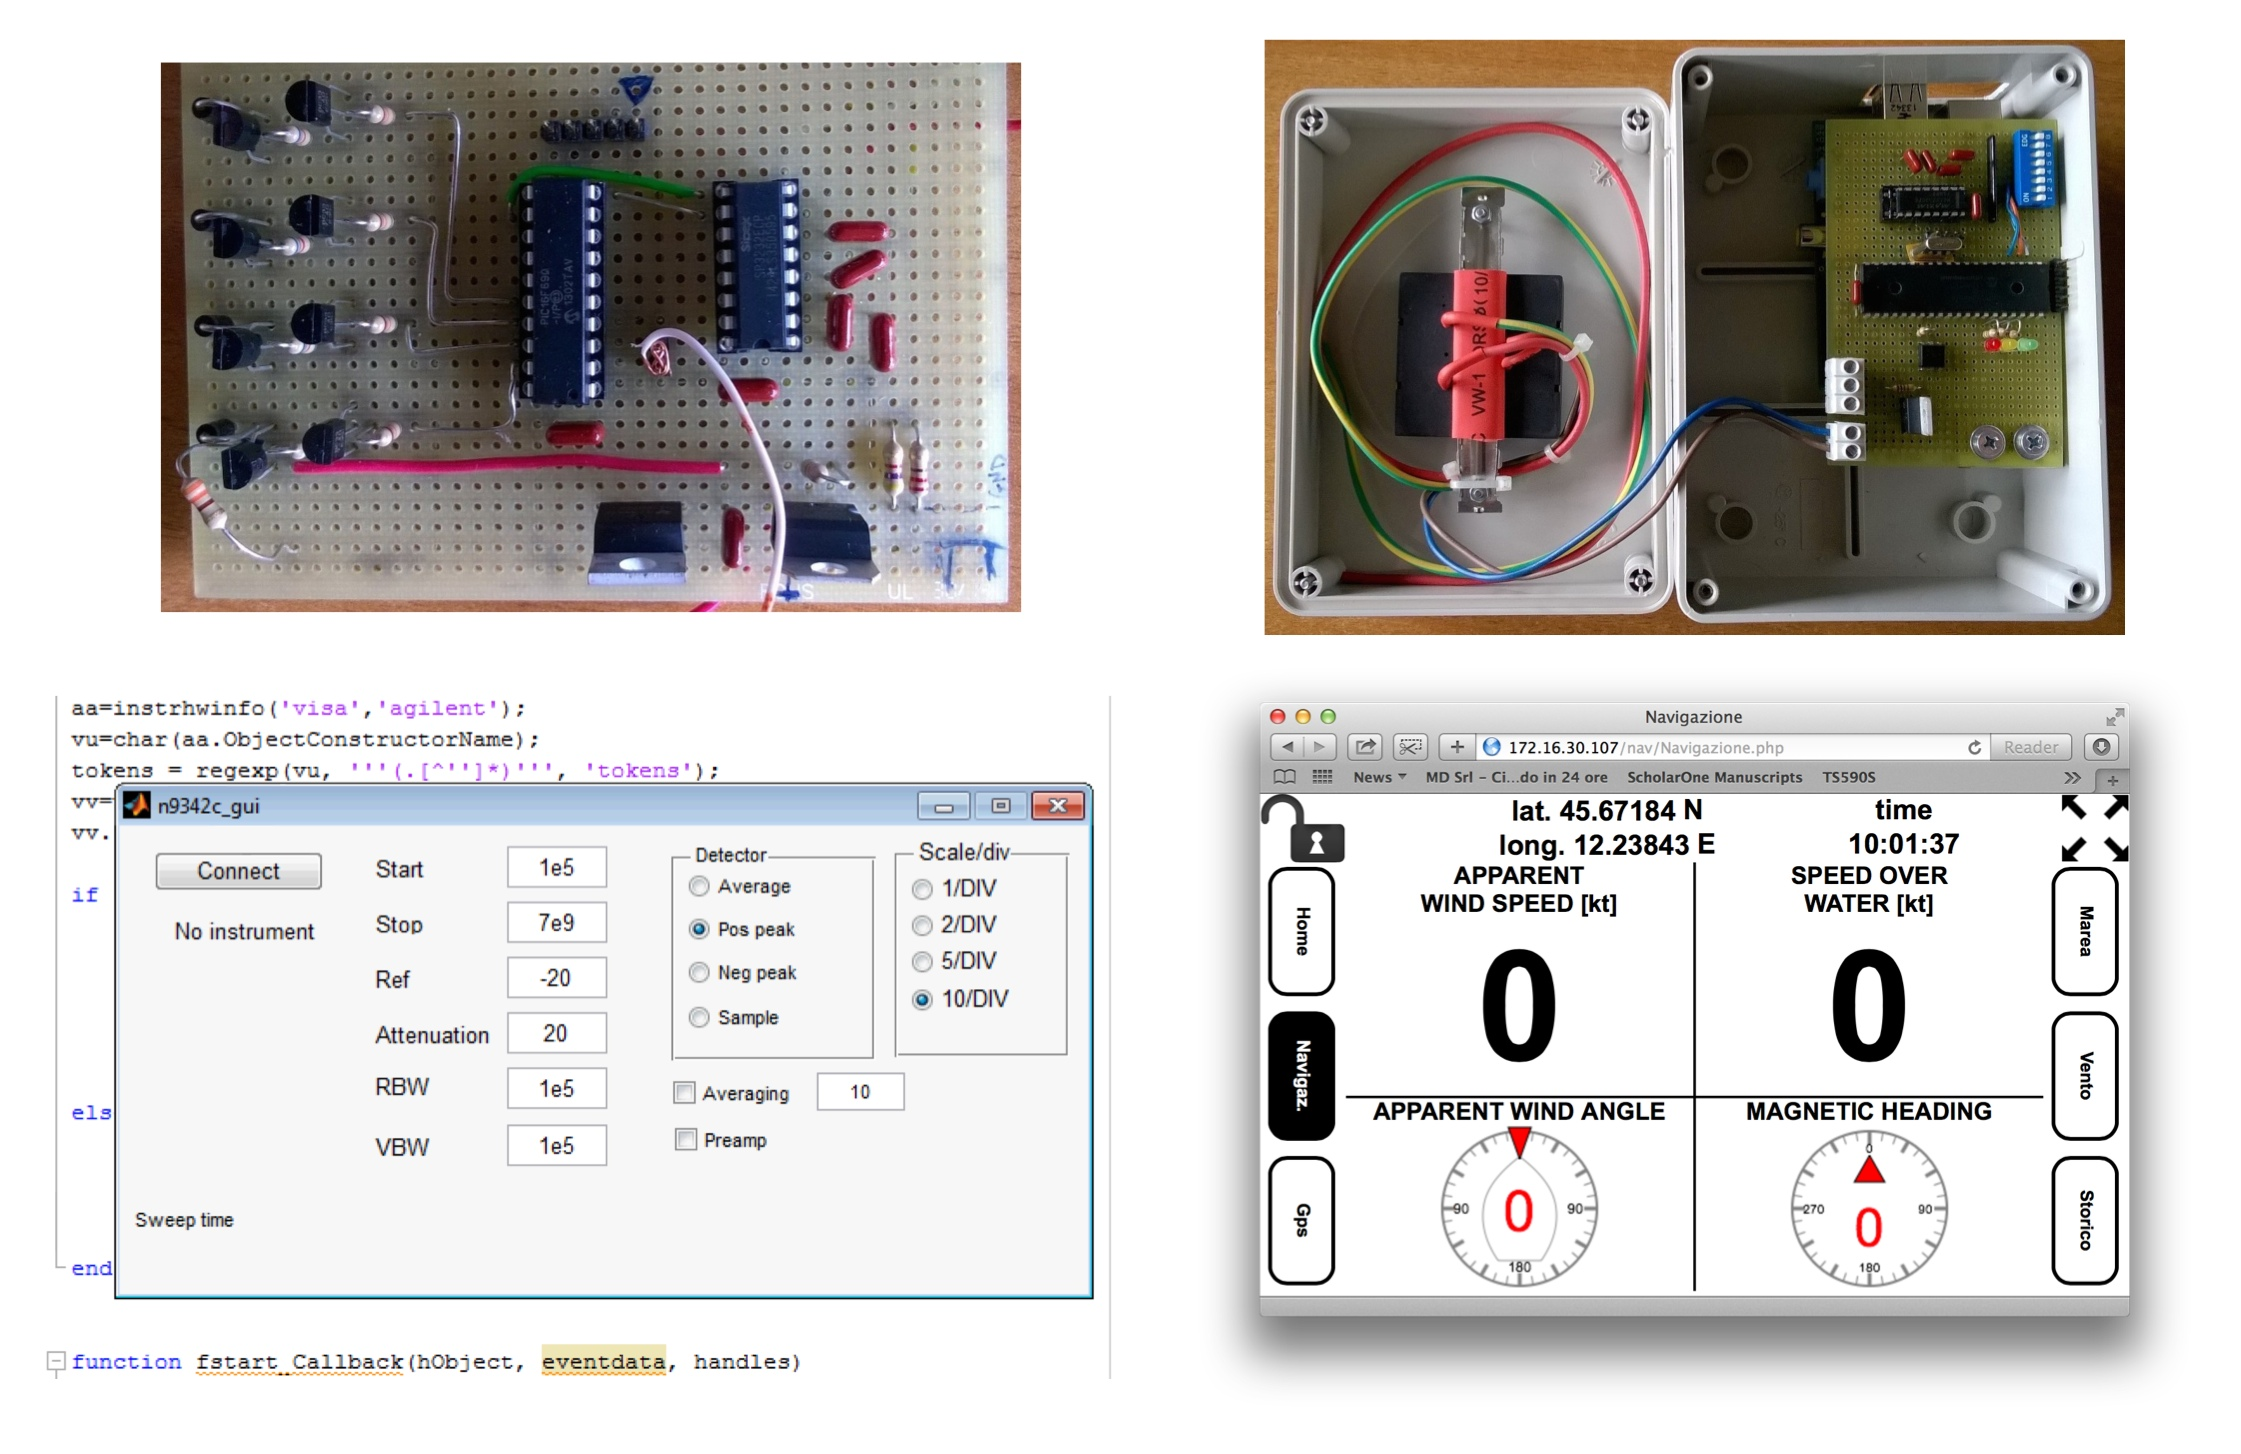
\includegraphics[width=0.8\textwidth]{img/emcy}
        \end{figure}
    \end{center}

    %\begin{minipage}{0.48\textwidth}
    %    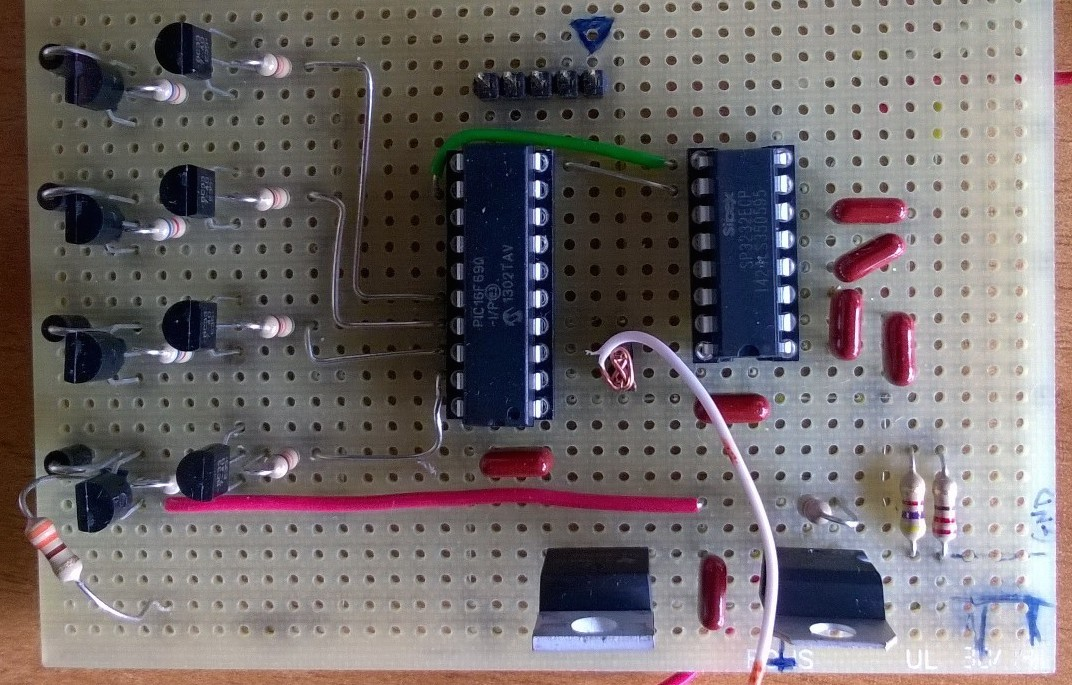
\includegraphics[width=\textwidth]{img/controller}
    %\end{minipage}
    %\begin{minipage}{0.48\textwidth}
    %    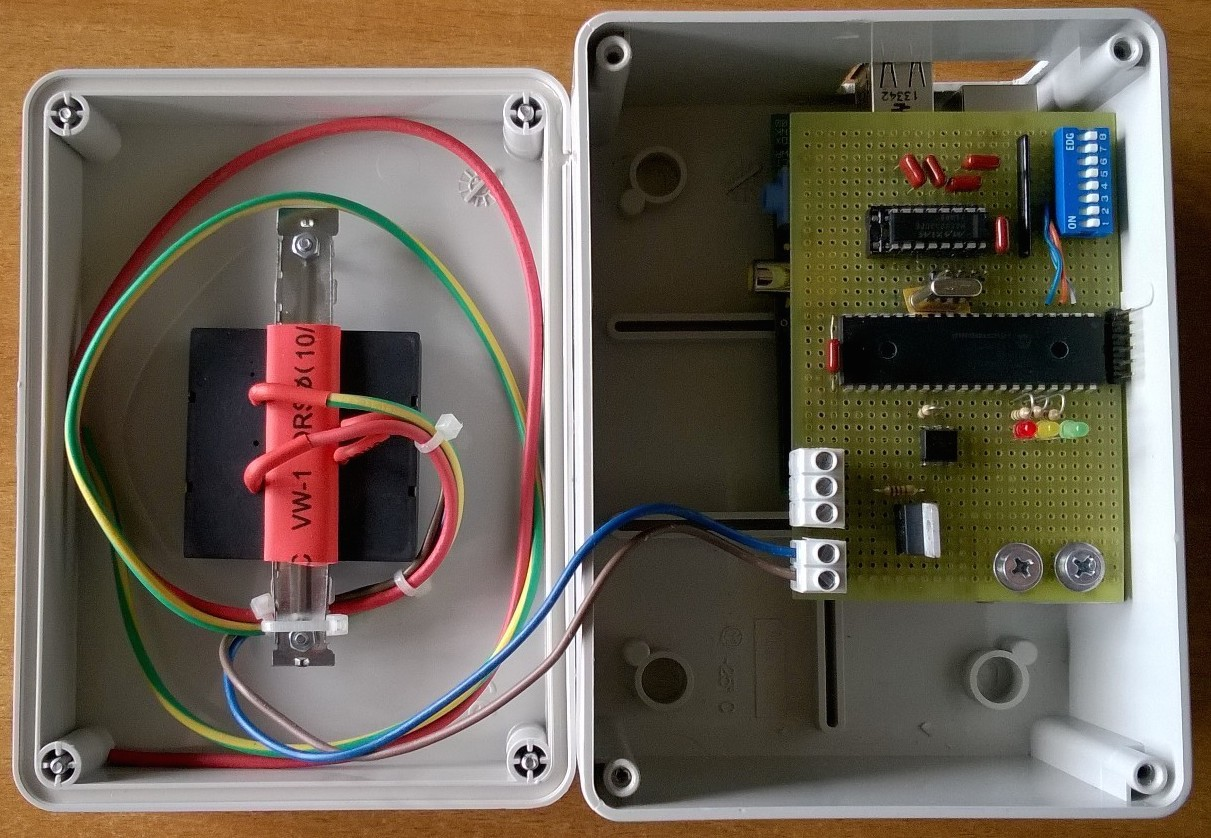
\includegraphics[width=\textwidth]{img/interface}
    %\end{minipage}
\end{frame}

%%%%%%%%%%%%%%%%%%%%%%%%%%%%%%%%%%%%%%%%%%%%%%%%%%%%
\begin{frame}{Training activity}
    \begin{itemize}
    \item Scientific skills training:
        \begin{itemize}
            \item \emph{Modelli numerici per campi e circuiti}, prof. F. Trevisan: 15 hours
            \item \emph{Propagazione e antenne}, prof. M. Midrio: 60 hours
            \item \emph{Elettrotecnica}, prof. F. Bellina: 90 hours
            \item  Tracks 1,2,3 e 4 compulsory courses: 72 hours
        \end{itemize}
    \item Applied training:
        \begin{itemize}
            \item PhD expo 2013, 2014 e 2015: 36 hours
            \item Seminar about EMT code: 1 hour
        \end{itemize}
        \begin{center}
            $\sum_i t_i = 274$ hours
        \end{center}

    \item Experimental activity at Emilab: about 16 hours/week.
    \end{itemize}


\end{frame}

%%%%%%%%%%%%%%%%%%%%%%%%%%%%%%%%%%%%%%%%%%%%%%%%%%%%
\begin{frame}{First year Gantt chart}

    \begin{center}
    \begin{tikzpicture}
        \begin{ganttchart}[canvas/.style=%
{fill=yellow!25, draw=blue, very thick},
y unit title=0.4cm,
            x unit=0.2cm,
            y unit chart=0.3cm,
            y unit title=0.3cm,
            vgrid,hgrid, 
            title label anchor/.style={below=-1.6ex},
            title left shift=.05,
            title right shift=-.05,
            title height=1,
            bar/.style={fill=blue!50},
            incomplete/.style={fill=white},
            progress label text={},
            bar height=0.7,
            group right shift=0,
            group top shift=.6,
            group height=.3,
            group peaks={}{}{.2}]{48}

          
                                    %labels
            \gantttitle{\tiny First year}{48} \\
            \gantttitle{\tiny Jan}{4} 
            \gantttitle{\tiny Feb}{4} 
            \gantttitle{\tiny Mar}{4} 
            \gantttitle{\tiny Apr}{4} 
            \gantttitle{\tiny Mai}{4} 
            \gantttitle{\tiny Jun}{4}
            \gantttitle{\tiny Jul}{4}
            \gantttitle{\tiny Aug}{4}
            \gantttitle{\tiny Sep}{4}
            \gantttitle{\tiny Oct}{4}
            \gantttitle{\tiny Nov}{4}
            \gantttitle{\tiny Dec}{4}
            
            \\

            %tasks
            \ganttbar{\tiny 1}{1}{8} \\
            \ganttbar{\tiny 2}{9}{22} \\
            \ganttbar{\tiny 3}{35}{48} \\
            \ganttbar{\tiny 4}{12}{20} \\
            \ganttbar{\tiny 5}{21}{24} \\
            \ganttbar{\tiny 6}{25}{30} \\
            \ganttbar{\tiny 7}{31}{34} \\
            \ganttbar{\tiny 8}{35}{48}
            %\ganttbar[progress=0]{\tiny 9}{41}{48}

        \end{ganttchart}
    \end{tikzpicture}
        \end{center}
        \begin{table}
            \footnotesize
            \centering
            \begin{tabular}{ll}
                1. \textcolor{red}{Modelli numerici per campi e circuiti} & 6. Solver integration\\
                2. \textcolor{red}{Propagazione e antenne} &  7. Software test\\
                3. \textcolor{red}{Elettrotecnica} & 8. Virtual device study\\
                4. Software implementation & \\% 9. Validazione sw e dispositivi \\
                5. Software test & \\
            \end{tabular}
        \end{table}
\end{frame}



%%%%%%%%%%%%%%%%%%%%%%%%%%%%%%%%%%%%%%%%%%%%%%%%%%%%
\begin{frame}{Second year Gantt chart}
        \begin{center}
    \begin{tikzpicture}

        \begin{ganttchart}[canvas/.style=%
{fill=yellow!25, draw=blue, very thick},
y unit title=0.4cm,
            x unit=0.2cm,
            y unit chart=0.3cm,
            y unit title=0.3cm,
            vgrid,hgrid, 
            title label anchor/.style={below=-1.6ex},
            title left shift=.05,
            title right shift=-.05,
            title height=1,
            bar/.style={fill=blue!50},
            incomplete/.style={fill=white},
            progress label text={},
            bar height=0.7,
            group right shift=0,
            group top shift=.6,
            group height=.3,
            group peaks={}{}{.2}]{48}

          
                                    %labels
            \gantttitle{\tiny Second year}{48} \\
            \gantttitle{\tiny Jan}{4} 
            \gantttitle{\tiny Feb}{4} 
            \gantttitle{\tiny Mar}{4} 
            \gantttitle{\tiny Apr}{4} 
            \gantttitle{\tiny Mai}{4} 
            \gantttitle{\tiny Jun}{4}
            \gantttitle{\tiny Jul}{4}
            \gantttitle{\tiny Aug}{4}
            \gantttitle{\tiny Sep}{4}
            \gantttitle{\tiny Oct}{4}
            \gantttitle{\tiny Nov}{4}
            \gantttitle{\tiny Dec}{4}
            
            \\

            %tasks
            \ganttbar[progress=100]{\tiny 1}{9}{48}\\
            \ganttbar[progress=100]{\tiny 2}{1}{24}\\
            \ganttbar{\tiny 3}{1}{6}\\
            \ganttbar{\tiny 4}{18}{19}\\
            \ganttbar[progress=100]{\tiny 5}{25}{48}

        \end{ganttchart}
    \end{tikzpicture}
        \end{center}
        \begin{table}
            \footnotesize
            \centering
            \begin{tabular}{ll}
                1. Experimental activity at Emilab &  4. CEFC2014  \\
                2. Software development & 5. Experimental validation of models \\
                3. \textcolor{red}{Elettrotecnica} \\
                
            \end{tabular}
        \end{table}
\end{frame}

%%%%%%%%%%%%%%%%%%%%%%%%%%%%%%%%%%%%%%%%%%%%%%%%%%%%
\begin{frame}{Third year Gantt chart}
        \begin{center}
    \begin{tikzpicture}

        \begin{ganttchart}[canvas/.style=%
{fill=yellow!25, draw=blue, very thick},
y unit title=0.4cm,
            x unit=0.2cm,
            y unit chart=0.3cm,
            y unit title=0.3cm,
            vgrid,hgrid, 
            title label anchor/.style={below=-1.6ex},
            title left shift=.05,
            title right shift=-.05,
            title height=1,
            bar/.style={fill=blue!50},
            incomplete/.style={fill=white},
            progress label text={},
            bar height=0.7,
            group right shift=0,
            group top shift=.6,
            group height=.3,
            group peaks={}{}{.2}]{48}

          
                                    %labels
            \gantttitle{\tiny Third year}{48} \\
            \gantttitle{\tiny Jan}{4} 
            \gantttitle{\tiny Feb}{4} 
            \gantttitle{\tiny Mar}{4} 
            \gantttitle{\tiny Apr}{4} 
            \gantttitle{\tiny Mai}{4} 
            \gantttitle{\tiny Jun}{4}
            \gantttitle{\tiny Jul}{4}
            \gantttitle{\tiny Aug}{4}
            \gantttitle{\tiny Sep}{4}
            \gantttitle{\tiny Oct}{4}
            \gantttitle{\tiny Nov}{4}
            \gantttitle{\tiny Dec}{4}            
            \\

            %tasks
            \ganttbar[progress=100]{\tiny 1}{1}{16}\\
            \ganttbar[progress=0]{\tiny 2}{26}{48}\\
            \ganttbar[progress=0]{\tiny 3}{24}{25}\\ 
            \ganttbar[progress=0]{\tiny 4}{25}{48}

        \end{ganttchart}
    \end{tikzpicture}
        \end{center}
        \begin{table}
            \footnotesize
            \centering
            \begin{tabular}{ll}
                1. Experimental activity at Emilab & 2. Thesis \\
                3. COMPUMAG2015 & 4. Experimental activity at Emilab
            \end{tabular}
        \end{table}
\end{frame}


%%%%%%%%%%%%%%%%%%%%%%%%%%%%%%%%%%%%%%%%%%%%%%%%%%%%
\begin{frame}{Thank you!}
    \begin{center}
        {\LARGE Thank you for your attention!}

        \vspace{1cm}
        \texttt{matteo.cicuttin@uniud.it}

        \vspace{1cm}
        {\Large Meet at poster session 16.30 - 19.00!}
    \end{center}
\end{frame}



\end{document}
